\documentclass[12pt,a4paper,oneside]{report}

\usepackage{fontspec}
\IfFontExistsTF{Calibri}{\setmainfont{Calibri}}{\setmainfont{Carlito}}
\usepackage[a4paper,margin=30mm,headheight=14pt,headsep=15mm]{geometry}
\usepackage{amsmath}
\usepackage{booktabs}
\usepackage{array}
\usepackage{setspace}
\usepackage[backend=biber,style=apa,natbib=true]{biblatex}
\addbibresource{references.bib}
\usepackage{graphicx}
\usepackage{xurl}
\usepackage{fvextra}
\DefineVerbatimEnvironment{verbatim}{Verbatim}{fontsize=\small,breaklines=true}
\usepackage{titlesec}
\usepackage{tocloft}
\usepackage{fancyhdr}
\usepackage{url}
\usepackage[hidelinks]{hyperref}

\onehalfspacing
\setlength{\emergencystretch}{3em}
\setlength{\tabcolsep}{2pt}
\setcounter{secnumdepth}{2}
\setcounter{tocdepth}{2}
\setcounter{biburlnumpenalty}{100}
\setcounter{biburllcpenalty}{100}
\setcounter{biburlucpenalty}{100}
\titleformat{\chapter}[hang]{\fontsize{16}{20}\selectfont\bfseries}{\thechapter}{1em}{}
\titleformat{\section}{\fontsize{14}{18}\selectfont\bfseries}{\thesection}{1em}{}
\titleformat{\subsection}{\fontsize{12}{16}\selectfont\bfseries}{\thesubsection}{1em}{}
\titlespacing*{\chapter}{0pt}{0pt}{18pt}
\renewcommand{\cftdotsep}{\cftnodots}
\setlength{\cftsecindent}{0.5cm}
\setlength{\cftsubsecindent}{1cm}
\pagestyle{fancy}
\fancyhf{}
\fancyhead[C]{\fontsize{11}{13}\selectfont\thepage}
\renewcommand{\headrulewidth}{0pt}
\fancypagestyle{plain}{\fancyhf{}\fancyhead[C]{\fontsize{11}{13}\selectfont\thepage}}

\title{Design and Implementation of a Hybrid Earth Observation Data Infrastructure\\
for Research and Education: A Case Study of Kvarken Space Center}
\author{Daniel Ebrahimzadeh Esfahani}
\date{2026}

\begin{document}

\begin{titlepage}
\thispagestyle{empty}
\centering

\includegraphics[width=55mm]{assets/uwasa-logo.jpg}\par
\vspace{25mm}
{\fontsize{16}{20}\selectfont Daniel Ebrahimzadeh Esfahani\par}
\vspace{10mm}
{\fontsize{20}{25}\selectfont\bfseries Design and Implementation of a Hybrid Earth Observation Data Infrastructure\par}
\vspace{5mm}
{\fontsize{14}{18}\selectfont for Research and Education: A Case Study of Kvarken Space Center\par}
\vspace{22mm}
\begin{flushright}
Master's Thesis\par
School of Technology and Innovations\par
Master's Degree Programme in Computing Sciences\par
Major: Artificial Intelligence and Data Engineering\par
Supervisor: Professor Ali Nadir Arslan\par
\end{flushright}
\vfill
Vaasa 2026\par
\end{titlepage}

\setcounter{page}{2}
\begingroup
\singlespacing
\fontsize{11}{12.5}\selectfont
\noindent\textbf{UNIVERSITY OF VAASA}\\
School of Technology and Innovations\\[4pt]
\begin{tabular}{@{}p{0.21\textwidth}p{0.75\textwidth}@{}}
Author & Däniel Ebrahimzadeh Esfahani\\
Title & Design and Implementation of a Hybrid Earth Observation Data Infrastructure for Research and Education: A Case Study of Kvarken Space Center\\
Degree & Master of Science in Technology\\
Programme & Computing Sciences; Artificial Intelligence and Data Engineering\\
Supervisor & Professor Ali Nadir Arslan\\
Year & 2026\\
\end{tabular}
\par\medskip\noindent\textbf{Abstract}\par

Earth Observation research depends on more than downloading satellite images. A usable
infrastructure must validate metadata, preserve the origin of observations, control external
requests, support spatial queries, and connect these operations to a scientific application.
This thesis designs and evaluates an in-house hybrid Earth Observation infrastructure to
support research and teaching within Kvarken Space Center and the University of Vaasa.
Here, hybrid means external standards-based data access combined with local persistence,
processing and an offline-safe engineering baseline.

The work follows an engineering design-and-evaluation approach. Provider responses are
validated before transformation into a transport-neutral scene model. The implementation
combines bounded active concurrency, content-addressed payload storage, append-only provenance,
an embedded spatial catalog, metadata quality filters and a read-only educational interface.
Students can use offline metadata fixtures, source validation, provenance inspection, spatial
queries, the read-only Application Programming Interface (API) and local real-data processing. These are implemented exercises;
learning outcomes were not evaluated.

The practical application examines sea-ice candidate mapping in eastern Kvarken using actual
Sentinel-1 radar observations and upstream CATALYST radiometric terrain-correction products
hosted by Microsoft Planetary Computer. Sentinel-2 observations provide conservative optical
proxy labels for snow-covered ice and dark water; European Space Agency (ESA) WorldCover 2021
v200 supplies an annual retrospective land mask, not a March 2021 ice observation. The overlapping records define a
single case rather than representative seasonal sampling. The optical scene followed the radar
acquisition, so proxy labels are not a contemporaneous reference. A scene-specific linear
discriminant uses both radar polarisations. Spatially separated training and evaluation blocks
avoid direct sample overlap. Outputs include georeferenced maps, quantitative reports and
checksummed acquisition records.

The engineering evaluation combines automated failure-oriented tests with a preserved
synthetic benchmark. The scientific application exposes a substantial limitation: positive
ice precision is low, and ordinary agreement is below an always-water baseline. Many candidate
cells have no optical reference labels, so the full candidate area is not validated sea-ice
extent. The acquisition gap, incomplete optical coverage, wind-sensitive radar backscatter,
unverified upstream noise treatment and untested illumination-angle effects limit
interpretation. The selected labelled cells support a diagnostic comparison only, not a
complete estimate of sea-ice conditions across the candidate area. Georeferenced maps and
acquisition records let the reader trace the relationship between the input observations and
the analysis. The experiment provides evidence of application integration, not an operational
ice-monitoring algorithm.

Raster analysis ran locally. A five-scene metadata replay on cPouta, a cloud service of the
Finnish IT Center for Science (CSC), verified scene identities,
persistent provenance, regional queries and the loopback API. This demonstrates a first-stage
remote research and teaching workflow, not image classification, distributed processing,
improved classifier accuracy or cloud scalability. Further independent observations and
educational evaluation remain future work.

\par\medskip\noindent\textbf{Keywords:} Earth Observation; Sentinel-1; sea ice; SpatioTemporal Asset Catalog;
provenance; spatial catalog; reproducibility; Kvarken
\endgroup

\tableofcontents
\clearpage
\listoffigures
\clearpage
\listoftables
\clearpage
\chapter*{Acknowledgements}

\addcontentsline{toc}{chapter}{Acknowledgements}

I would like to thank my parents for their support.

I would like to thank Professor Ali Nadir Arslan for the supervision and scientific direction of this thesis and the Kvarken Space Center context for giving the work a concrete research setting. I also thank the University of Vaasa for providing an academic environment in which software engineering, Earth Observation, and reproducible research can be studied together.

The practical orientation of this work reflects my interest in building systems that are technically clear, maintainable, and useful to other researchers. I am grateful to the people who supported the development, review, and completion of the thesis.

\chapter*{Abbreviations}

\addcontentsline{toc}{chapter}{Abbreviations}

\small
\begin{longtable}{p{0.27\textwidth}p{0.66\textwidth}}
\toprule
\textbf{Abbreviation} & \textbf{Meaning} \\
\midrule
\endfirsthead
\toprule
\textbf{Abbreviation} & \textbf{Meaning} \\
\midrule
\endhead
ACID & Atomicity, Consistency, Isolation, and Durability \\
AI & Artificial Intelligence \\
APA & American Psychological Association \\
API & Application Programming Interface \\
AWS & Amazon Web Services \\
CDSE & Copernicus Data Space Ecosystem \\
CI & Continuous Integration \\
CLI & Command-Line Interface \\
COG & Cloud-Optimized GeoTIFF \\
CPU & Central Processing Unit \\
CRS & Coordinate Reference System \\
CSC & Finnish IT Center for Science \\
CSL & Citation Style Language \\
CUDA & Compute Unified Device Architecture \\
DEA & Digital Earth Australia \\
EO & Earth Observation \\
EPSG & Identifier in the EPSG Geodetic Parameter Dataset \\
ESA & European Space Agency \\
F1 & F-score, the harmonic mean of precision and recall \\
GDAL & Geospatial Data Abstraction Library \\
GIS & Geographic Information System \\
GPU & Graphics Processing Unit \\
GRDH & Ground Range Detected, High Resolution \\
HTTP & Hypertext Transfer Protocol \\
I/O & Input/output \\
IP & Internet Protocol \\
IW & Interferometric Wide swath \\
JSON & JavaScript Object Notation \\
NASA & National Aeronautics and Space Administration \\
NDSI & Normalized Difference Snow Index \\
NDVI & Normalized Difference Vegetation Index \\
OAuth2 & OAuth 2.0 authorization framework \\
OData & Open Data Protocol \\
ODC & Open Data Cube \\
OGC & Open Geospatial Consortium \\
PDF & Portable Document Format \\
PDF/A & Archival subset of the Portable Document Format \\
REST & Representational State Transfer \\
RQ & Research question identifier \\
RTC & Radiometrically Terrain Corrected \\
S3 & Simple Storage Service-compatible object access interface \\
SAFE & Standard Archive Format for Europe \\
SAR & Synthetic Aperture Radar \\
SAS & Shared Access Signature \\
SCL & Sentinel-2 Scene Classification Layer \\
SDK & Software Development Kit \\
SHA-256 & Secure Hash Algorithm 256-bit digest \\
SNAP & Sentinel Application Platform \\
SQL & Structured Query Language \\
SSH & Secure Shell \\
STAC & SpatioTemporal Asset Catalog \\
SWIR & Short-wave infrared \\
URI & Uniform Resource Identifier \\
URL & Uniform Resource Locator \\
UTC & Coordinated Universal Time \\
UTF-8 & 8-bit Unicode Transformation Format \\
UTM & Universal Transverse Mercator \\
VH & Vertical transmit, horizontal receive polarization \\
VM & Virtual Machine \\
VRAM & Video Random-Access Memory \\
VV & Vertical transmit, vertical receive polarization \\
WAL & Write-Ahead Logging \\
WGS 84 & World Geodetic System 1984 \\
\bottomrule
\end{longtable}
\normalsize

\clearpage

\chapter{Introduction}

\section{Motivation and research context}

Earth Observation (EO) has become an important source of information for research, environmental monitoring, regional analysis, and teaching. Satellite missions such as Sentinel-2 provide multispectral observations suitable for land-cover and vegetation analysis \citep{drusch2012sentinel}. Scientific use of these observations, however, depends on more than access to image files. Researchers must identify products, interpret metadata, manage spatial and temporal constraints, preserve provenance, cope with provider failures, and retain a processing path that can be repeated later.

These requirements create a data-engineering problem. A research group may have access to public EO services but still lack a compact infrastructure that connects provider access, validation, storage, spatial indexing, controlled processing, and reproducible reporting. Large cloud platforms can provide substantial capability, but a university research environment may also need a local path that remains understandable, auditable, and usable when credentials or network access are unavailable. The engineering challenge is therefore not simply to download satellite products. It is to construct a trustworthy path from an external provider response to a research-ready and traceable local representation.

The Kvarken Space Center provides the contextual setting for this thesis. The implementation uses a predefined Kvarken study region and focuses on requirements relevant to a small research and educational environment: standards-based access, reproducibility, transparent failure handling, modest infrastructure requirements, and the ability to demonstrate the processing path without depending on a live production service. The thesis does not evaluate the organizational performance of Kvarken Space Center or student learning outcomes. The case-study framing therefore refers to the institutional and regional context used to motivate and bound the artifact.

\section{Problem statement and research gap}

Standards and public platforms address important parts of EO access. STAC provides a common JSON-based description of spatiotemporal assets, OGC standards support interoperable geospatial interfaces, and the Copernicus Data Space Ecosystem (CDSE) provides access to Copernicus data and cloud-oriented processing services \citep{ogc-api-features,stac-spec,cdse,kovacs2026cdse}. These facilities reduce fragmentation at the provider boundary, but they do not by themselves define how a small research project should validate incoming metadata, preserve raw evidence, bound concurrent work, separate transient from permanent failures, maintain a local spatial catalog, or freeze empirical artifacts for later comparison.

Within the scope of this thesis, the research gap is therefore operational and architectural rather than a claim that equivalent technologies do not exist. The question is how standards-based provider access can be assembled into a small, reproducible, and inspectable research infrastructure with explicit contracts. The system must be usable both with external providers and deterministic offline fixtures. It must avoid hidden retry behavior, unbounded task creation, silent coordinate-system assumptions, and mutable experiment evidence.

\section{Objective and scope}

The objective is to design, implement, and evaluate a hybrid EO data infrastructure that connects external standards-based access with local reproducible storage and processing. In this thesis, \emph{hybrid} refers to that combination of external provider access and local research infrastructure, including an offline execution path based on checked-in fixtures.

The implemented scope includes STAC/CDSE access concepts, typed validation, a provider-neutral \texttt{EOScene} model, OAuth2 token handling, bounded asynchronous ingestion, SHA-256 content addressing, append-only provenance, a SQLite/WAL spatial catalog, metadata quality profiling, a range-based raster/NDVI slice, deterministic experiment reports, and a read-only educational HTTP interface.

The evaluation now includes an executed Sentinel-1 sea-ice application in the eastern Kvarken study rectangle. Actual calibrated radar pixels are compared with conservative labels derived from a separate Sentinel-2 acquisition. This extends the infrastructure evaluation to raster decoding, common-grid processing, land exclusion, classification, and sensor-independent reference agreement. It does not establish field-validated sea-ice accuracy, production CDSE performance, distributed scalability, or educational learning outcomes. An actual CSC cPouta demonstration is required for the revised review package but has not yet been executed because authenticated project access is unavailable to this session.

\section{Research questions}

\begin{enumerate}
  \item How can heterogeneous STAC and CDSE metadata be validated and transformed into a transport-neutral EO scene model while preserving provenance?
  \item How can asynchronous ingestion remain bounded and recover from transient timeouts, OAuth2 expiration, and HTTP 429 responses without retrying malformed payloads?
  \item How effectively can a dependency-free SQLite catalog support regional, temporal, quality, and platform queries under concurrent reader/writer contention?
  \item Which empirical measurements and artifacts are sufficient to make an offline EO pipeline baseline reproducible for research and education?
  \item Can the infrastructure support a traceable real-data sea-ice application, and what does comparison with independent optical evidence reveal about its scientific limitations?
\end{enumerate}

\section{Contributions}

The thesis makes four related contributions. First, it defines an architectural baseline in which provider-specific behavior is isolated from a typed domain model. Second, it implements an engineering artifact that combines bounded concurrency, provenance, embedded spatial persistence, quality filtering, lightweight raster analysis, and a read-only educational interface. Third, it defines a reproducibility protocol based on frozen fixtures, deterministic reports, versioned source, CI, and dated additive experiment artifacts. Fourth, it makes the limits of the evidence explicit so that synthetic benchmark results are not presented as production-provider performance.

The contribution is architectural and methodological rather than a new remote-sensing algorithm. The application also tests an important boundary: an infrastructure can run correctly while its scientific classifier remains unsuitable for operational extent estimation. Reporting both outcomes is more informative than treating a successful processing command as scientific validation.

\section{Structure of the thesis}

Chapter 2 reviews the EO standards, provider context, provenance, and embedded persistence concepts used by the system. Chapter 3 explains the research methodology and evidence strategy. Chapter 4 presents the architecture and its invariants. Chapter 5 documents implementation and the real-data application. Chapter 6 reports the synthetic baseline and observed satellite results separately. Chapter 7 analyzes the research questions. Chapter 8 discusses contributions and validity. Chapter 9 concludes the thesis and identifies remaining work.

\chapter{Background}

\section{Radar sea ice and independent optical evidence}

Synthetic Aperture Radar (SAR) observations support sea-ice monitoring, but a radar return is a measurement of
scattering properties rather than a direct semantic ice label. Ice-type classification,
motion retrieval and melt detection are distinct tasks; combining active and passive
sensors can provide complementary evidence \citep{dierking2013}. This thesis uses
dual-polarisation Sentinel-1 for one exploratory classification task, not all of these
capabilities.

Radiometric terrain correction normalises geometric influences on observed brightness
\citep{small2011}. It does not by itself identify sea ice. The practical experiment therefore
uses independent Sentinel-2 reflectance and scene categories to construct a selective
reference. The optical label rules are explicit experimental assumptions, not field
observations. Different sensor times, incomplete coverage and uncertain classes must
remain visible in interpretation. An operational ice chart can be informative but is
not necessarily independent when its production already uses Sentinel-1.

\section{Earth observation information models}

Earth observation (EO) systems produce observations whose scientific value depends on both the
measurement and its context. A pixel array without acquisition time, spatial reference, processing
level, or a stable identifier is difficult to search, compare, or reproduce. This thesis therefore
treats metadata as a first-class data product. The representative mission is Sentinel-2, whose
multispectral instrument provides bands suitable for land-cover and vegetation analysis
\cite{drusch2012sentinel}. The architectural problem is not only downloading imagery; it is
maintaining a verifiable chain from a provider record to a queryable, quality-assessed research
scene.

\section{Comparative EO access and processing environments}

Several established services already provide EO discovery, data access, and processing. This
thesis does not treat the absence of a global platform as a research gap. Its narrower question
is how a small University of Vaasa research and teaching project can keep provider access,
validation, provenance, local queries, and offline reproduction inspectable while using external
data and compute services where they are useful. Table~\ref{tab:eo-platforms} compares the
principal alternatives by service model, data and processing access, portability, and likely
fit for a CSC-hosted student workflow. The educational and CSC assessments are design analysis;
they are not comparative usability tests.

An application programming interface (API) is a contract exposed by a service, not necessarily
a data archive or a compute environment. Cloud Optimized GeoTIFF (COG) is a file layout that
supports range-based access; it does not itself provide catalogue search or processing.
Consequently, a platform name can describe a catalogue, hosted compute, a standard, or a
software ecosystem. These categories should not be conflated when evaluating portability or
onboarding.

\small
\begin{longtable}{p{0.15\textwidth}p{0.27\textwidth}p{0.29\textwidth}p{0.20\textwidth}}
\caption{Comparison of EO platforms, standards, and software ecosystems}
\label{tab:eo-platforms}\\
\toprule
\textbf{Service or ecosystem} &
\textbf{Data access and processing} &
\textbf{Standards, provenance, access, and ownership} &
\textbf{Research, education, and CSC fit} \\
\midrule
\endfirsthead
\multicolumn{4}{c}{\tablename\ \thetable{} -- continued from previous page}\\
\toprule
\textbf{Service or ecosystem} &
\textbf{Data access and processing} &
\textbf{Standards, provenance, access, and ownership} &
\textbf{Research, education, and CSC fit} \\
\midrule
\endhead
\midrule
\multicolumn{4}{r}{Continued on next page}\\
\endfoot
\bottomrule
\endlastfoot

\textbf{Copernicus Data Space Ecosystem (CDSE)} &
Provides Copernicus mission data through services including STAC, the Open Data Protocol
(OData), Simple Storage Service (S3)-compatible object access, openEO, and
Sentinel Hub APIs. Processing can be remote through supported services; users can also retrieve
assets for external compute \citep{cdse,cdse-quotas,kovacs2026cdse}. &
European Commission/Copernicus infrastructure with account-based services and documented
quota controls. STAC and openEO provide standard interfaces, but processing support and limits
depend on the selected service. Provenance must retain item identifiers, process parameters,
and service-specific context. &
Strong public-data option for European EO exercises. CSC can call external APIs or host
downstream analysis, subject to account access, network policy, and quota. This thesis tests
CDSE adapters offline only; it does not verify a live CDSE request. \\

\textbf{Google Earth Engine} &
Offers a large curated multi-mission catalogue and server-side geospatial analysis through its
Code Editor, client libraries, and Representational State Transfer (REST) API. It removes much local data preparation for many
workflows, but users work within the hosted service's supported data and processing model
\citep{gee-paper,gee-access}. &
Google-owned service requiring a Google Cloud project with the Earth Engine API enabled,
registration for commercial or noncommercial use, and appropriate permissions. Scripts and
asset identifiers support traceability, but the hosted runtime and catalogue are not a
portable local execution environment. Terms and limits vary with account use. &
The interactive editor can lower the first barrier to exploratory teaching. Project
registration, usage terms, and service dependence add onboarding steps. A CSC workflow could
use the API, but it would still depend on Google authentication and remote execution; no such
integration was tested here. \\

\textbf{Microsoft Planetary Computer} &
Combines a STAC catalogue with cloud-hosted open datasets and asset access patterns suitable
for partial reads, including COGs. Processing can use client-side tools and external or
cloud-hosted compute; the catalogue and signed asset access should not be mistaken for a
guaranteed general-purpose compute allocation \citep{pc-about,pc-s1-rtc}. &
Microsoft-hosted data services expose open metadata and file formats, while access signing
and service availability remain provider-controlled. The documentation identified the public
service as a preview at the time checked, so feature status and terms must be rechecked.
Reproduction should record collection, item, asset, processing version, and access date. &
Useful for a reproducible case study because item metadata and COG assets can be inspected
and selected windows can be read without a full local download. The thesis used it to obtain
the case-study pixels for local analysis, not as evidence of CSC raster processing or
provider-independent compute. \\

\textbf{CREODIAS} &
Combines an EO product repository and data-exploration tools with CloudFerro cloud storage
and computing. Its documented services include S3-based remote data transfer and product
generation as a service; collection coverage and service features depend on the current
catalogue and product \citep{creodias-overview}. &
The infrastructure is operated as a commercial cloud service with user accounts and
service-specific terms. Published pricing can support cost estimation, but storage, compute,
and transfer costs depend on configuration. APIs and data formats should be checked for each
service rather than assumed to be interchangeable with CDSE or CSC. &
Potentially suitable for end-to-end EO labs where an integrated archive and processing
environment are important. It requires a separate provider account and cost controls.
Porting a containerized workflow to CSC is plausible, but data locality, quotas, and
performance were not evaluated in this thesis. \\

\textbf{openEO API and hosted backends} &
The openEO API specifies client-to-backend operations for data cubes and process graphs; it
is an interface standard, not a single archive or hosted platform. Multiple providers list
their own backends, collections, supported processes, and compute environments
\citep{openeo-paper,openeo-docs,openeo-backends}. &
R, Python, and JavaScript clients can express workflows against a common API. Authentication,
resource limits, job handling, data availability, and provenance details remain backend
specific. Process graphs help communicate intent, but equivalent results still depend on
collection versions, process support, parameters, and backend behavior. &
The shared client model is useful for teaching the distinction between workflow intent and
provider execution. It can reduce service-specific client code, but does not remove account
setup or backend limits. No openEO client or backend was exercised on CSC for this thesis. \\

\textbf{Pangeo} &
Pangeo is a community and software ecosystem for open, reproducible, scalable geoscience,
including tools such as xarray, Dask, and Zarr. It is not an EO archive. Users connect those
tools to separately hosted collections and compute \citep{pangeo-paper,pangeo-home}. &
Open-source software supports inspectable environments and cloud-native data access, but
there is no single Pangeo identity, quota, catalogue, or provenance service. Deployment,
authentication, storage ownership, and cost are set by the institution or cloud operator. &
Flexible for research and advanced data-engineering education, but students need environment
management and compute support. CSC could host compatible software, subject to service
configuration and allocations. This is a possible deployment route, not an implemented
dependency of the Kvarken prototype. \\

\textbf{Open Data Cube (ODC)} &
ODC is open-source software for indexing and analysing EO data; it is not itself a global
archive. A deployment ingests or indexes selected datasets and can use distributed processing.
Digital Earth Australia is an example of an operational national service using a related
data-cube approach \citep{odc-home,dea-home}. &
The open software permits local control over schemas and processing, while the operator owns
the catalogue, storage, authentication, backup, and compute lifecycle. Standards-based data
formats can help exchange, but deployment-specific metadata and ingestion conventions still
need to be recorded. &
Suitable where a group needs persistent, domain-curated datasets and can maintain the
service. It has more operational setup than the embedded SQLite catalogue used here. A CSC
deployment could be studied, but this thesis did not install or benchmark ODC. \\
\end{longtable}
\normalsize

The comparison shows what an in-house system should reuse. Public catalogues and standards
already solve much of data discovery and access; hosted platforms also supply scaled processing.
The prototype therefore reuses STAC metadata, OGC interfaces, OAuth2, open raster formats,
the provider's CATALYST RTC product, and Planetary Computer-hosted assets. It implements
project-specific schema checks, transport-neutral scene records, bounded active concurrency,
explicit retry classification, content-addressed source storage, append-only provenance, a
local SQLite spatial catalogue, offline reports, and a read-only educational API. It does not
reimplement a global catalogue, remote raster service, or cloud scheduler.

Several related services occupy distinct positions. The National Aeronautics and Space
Administration (NASA) Earthdata system provides access to NASA mission holdings and
authentication through Earthdata Login \citep{nasa-earthdata}. Digital Earth Australia (DEA)
is a curated national data service built around Australian satellite observations and
analysis-ready products \citep{dea-home,odc-home}. The European Space Agency (ESA)
EarthCODE programme focuses on discoverable and citable Earth-science experiments and
workflows, rather than acting as a general replacement for mission archives
\citep{esa-earthcode}. The Amazon Web Services (AWS) Open Data Registry lists datasets
hosted on AWS; its presence does not make AWS the data owner or remove the need to assess
compute and transfer costs \citep{aws-registry}. UP42 provides a commercial marketplace and
workflow services across multiple data providers \citep{up42-home}.

The name Sentinel Hub requires particular care. CDSE exposes Sentinel Hub APIs within its
Copernicus service portfolio. Planet separately markets Sentinel Hub capabilities as part of
its commercial Planet Insights Platform after acquiring the Sentinel Hub business. Shared
service history does not make CDSE access terms and Planet commercial terms interchangeable
\citep{cdse-sentinelhub,planet-insights}. Neither Sentinel Hub service is the source of the
Sentinel-1 raster assets in this thesis.

For the University and Kvarken Space Center, the in-house contribution is the explicit path
from offline exercises to a first remote metadata prototype, not superiority over these
platforms. The five-scene CSC cPouta run stored authentic captured metadata with provenance,
queried the SQLite catalogue, and exercised a loopback API. CSC did not perform live catalogue
discovery, fetch the raster windows, or run the scientific classifier. A student workflow can
teach validation and traceability with the existing exercises, while live provider use,
CSC raster work, multi-user operations, cost comparison, and learning outcomes remain outside
the demonstrated scope. The next section specifies the STAC records and asset relationships
that the prototype consumes.

\section{STAC's hierarchical catalog model}

The SpatioTemporal Asset Catalog (STAC) specification provides a JSON-based vocabulary for
describing geospatial information \cite{stac-spec}. Its hierarchy separates collection-level
description from observation-level metadata:

\begin{description}
\item[Catalog] A navigational root or subcatalog that groups related resources through typed
links. A catalog can expose multiple collections without prescribing how the data are stored.
\item[Collection] A logical set of Items sharing a mission, product family, or processing
definition. Collection metadata describes the spatial and temporal extent, license, providers, and
available summaries.
\item[Item] A single spatiotemporal observation. It has a globally meaningful identifier,
acquisition timestamp, GeoJSON geometry, bounding box, and properties such as platform and cloud
cover. Items are the unit transformed into the pipeline's typed \texttt{EOScene}.
\item[Asset] A link to a concrete downloadable resource, such as a spectral band, quicklook, or
metadata document. Asset roles and media types allow clients to distinguish data required for
analysis from ancillary resources.
\end{description}

The distinction between an Item and its Assets is operationally important. Search can remain
metadata-only, while an analytical task selectively fetches only the bands it needs. A normalized
scene can consequently be represented as
\[
 S = (i, p, t, g, b, a, q),
\]
where \(i\) is the item identifier, \(p\) the platform, \(t\) the acquisition instant, \(g\) the
geometry, \(b\) the bounding box, \(a\) the asset map, and \(q\) optional quality metadata. The
pipeline validates this tuple before persistence, preventing malformed provider payloads from
becoming catalog state.

\section{CDSE provider architecture and authorization}

The Copernicus Data Space Ecosystem (CDSE) exposes Copernicus data products and services through
provider-facing APIs \cite{cdse}. In this project, CDSE is an external boundary rather than a
dependency of the domain model. The asynchronous STAC client consumes search responses, while the
OAuth2 adapter obtains an access token and supplies it to subsequent metadata requests.
The implemented \texttt{CDSEClient} and token-provider interfaces have been exercised with
injected offline transports only. The tests do not contact CDSE, and the repository contains no
confirmed successful live CDSE metadata search. A previously recorded unauthenticated raster
request returned HTTP 401; no CDSE pixel download is confirmed. The raster asset code does not
implement or test an authenticated CDSE pixel-download workflow.

The client-credentials flow is appropriate for a non-interactive service account. Let \(c\) be the
client identifier, \(s\) the client secret, and \(u_t\) the token endpoint. The provider receives a
form request equivalent to
\[
 (c, s, \texttt{grant\_type}=\texttt{client\_credentials}) \longrightarrow
 (\texttt{access\_token}, \texttt{expires\_in}).
\]
The token is then sent as an HTTP bearer credential:
\[
\texttt{Authorization: Bearer <access\_token>}
\]
Secrets are resolved from environment variables and never placed in source code, reports, or
provenance manifests. A missing or incomplete configuration selects the offline fixture transport,
which makes tests and teaching exercises deterministic.

The token cache must distinguish validity from mere presence. If \(t_{\mathrm{now}}\) is the
current time, \(t_{\mathrm{issued}}\) the acquisition time, \(L\) the provider lifetime, and
\(\delta\) a refresh skew, a cached token is usable only when
\[
t_{\mathrm{now}} < t_{\mathrm{issued}} + \max(0, L-\delta).
\]
Refreshing before the nominal expiry avoids starting a long search with a token that expires while
the request is in flight. Network timeouts and HTTP 429 responses are transient; malformed token
JSON, an absent token, or a non-positive lifetime are permanent protocol errors.

\section{Geospatial filtering and indexing}

The Kvarken region is first approximated in the World Geodetic System 1984 (WGS 84)
coordinate reference system (CRS) by an axis-aligned bounding box
\[
B_R=[\lambda_{\min},\lambda_{\max}]\times[\phi_{\min},\phi_{\max}]
=[20.5,22.5]\times[62.8,63.8].
\]
For an Item bounding box \(B_S=[\lambda^-_S,\lambda^+_S]\times[\phi^-_S,\phi^+_S]\), the
necessary intersection predicate is
\[
\lambda^-_S\leq\lambda^+_R \land
\lambda^+_S\geq\lambda^-_R \land
\phi^-_S\leq\phi^+_R \land
\phi^+_S\geq\phi^-_R.
\]
This inexpensive predicate is suitable for indexed Structured Query Language (SQL) columns. It is a pre-filter, not a complete
topological test: two bounding boxes can overlap even when their polygons do not.

The exact second-stage test uses polygon intersection. For point-in-polygon classification, the
ray-casting algorithm counts crossings of a horizontal ray from point \(P=(x,y)\). For every edge
\((x_i,y_i)\) to \((x_j,y_j)\), a crossing is counted when
\[
(y_i>y)\mathbin{\ne}(y_j>y)
\quad\land\quad
x < x_i + \frac{(y-y_i)(x_j-x_i)}{y_j-y_i}.
\]
The point is inside when the crossing count is odd:
\[
\operatorname{inside}(P)=\left(\sum_i \operatorname{cross}_i(P)\right)\bmod 2=1.
\]
Boundary points are treated as intersecting so that observations touching the regional boundary are
not silently excluded. The implementation keeps this deterministic geometry logic separate from
HTTP transport and SQL access.

\section{Embedded persistence and SQLite WAL}

SQLite is an embedded relational database with transactional durability and no separate server
process. The catalog stores stable scene identity, platform, acquisition time, cloud cover,
bounding-box coordinates, serialized geometry, and serialized assets. B-tree indexes reduce the
candidate set before exact spatial checks; an idempotent primary-key upsert makes repeated
ingestion safe.

Write-ahead logging (WAL) changes the commit path: a writer appends changed pages to a WAL file
and readers continue from a consistent snapshot of the main database plus the WAL
\cite{sqlite-wal}. A reader that begins at snapshot \(r\) does not observe later commits until it
starts a new transaction. Consequently, concurrent readers can see different valid counts during a
write burst, but no reader should observe a half-written row. Checkpointing eventually transfers
committed pages back to the main database.

The durability contract follows the Atomicity, Consistency, Isolation, and Durability (ACID)
properties:
\begin{description}
\item[Atomicity] A scene upsert commits as one transaction; an error rolls back the complete
transaction rather than exposing a partial record.
\item[Consistency] primary-key, type, and application-level geometry invariants hold before and
after each commit.
\item[Isolation] readers see a stable committed snapshot and never uncommitted writer state.
\item[Durability] after a successful commit and connection close, reopening the catalog recovers
the committed rows, including rows written while WAL was active.
\end{description}

SQLite's connection objects are not freely shareable across threads. The project uses a
process-local reentrant lock around operations on the shared catalog connection, explicit
transactions for writes, and WAL to reduce reader--writer blocking. This is an ownership boundary,
not a substitute for distributed coordination: multiple processes require separate connections and
deployment-level locking decisions.

\section{Reproducibility and operational standards}

The OGC API Features model reinforces the separation between interoperable feature access and
provider-specific storage \cite{ogc-api-features}. In the thesis pipeline, reproducibility is
implemented through typed boundary validation, canonical JSON serialization, SHA-256 content
addresses, append-only manifests, deterministic reports, and frozen benchmark artifacts. These
controls make a synthetic experiment inspectable without a cloud service while leaving a clear
boundary for authenticated CDSE experiments.

\chapter{Methodology}

\section{Research design}

This thesis uses a design-and-evaluation engineering approach. The approach is descriptive rather than a claim that the project followed a specific named design-science framework. The research questions identify architectural properties that must be achieved; these properties are translated into implementation invariants; the invariants are realized in software; and the resulting artifact is evaluated with deterministic tests, a controlled synthetic benchmark, and preserved experiment records.

This framing is important because the central research object is an infrastructure artifact. The thesis cannot answer its questions only by describing code, and it cannot evaluate the system only by reporting a single throughput number. Evidence is therefore divided into four classes: structural evidence from architecture and source contracts, behavioral evidence from tests, performance evidence from the frozen benchmark, and reproducibility evidence from versioned fixtures and artifacts.

\section{Research questions and evidence mapping}

\begin{table}[htbp]
\centering
\caption{Research questions, primary evidence, and claim boundaries}
\small
\begin{tabular}{p{0.08\textwidth}p{0.24\textwidth}p{0.31\textwidth}p{0.28\textwidth}}
\toprule
\textbf{RQ} & \textbf{Primary evidence} & \textbf{What the evidence supports} & \textbf{What it does not support} \\
\midrule
RQ1 & Boundary validation, \texttt{EOScene} transformation, provenance records, schema tests & Provider-neutral normalization with traceable source evidence & Universal compatibility with all EO providers or schemas \\
RQ2 & Bounded ingestor, timeout/429/token tests, explicit error classes & Controlled recovery and bounded active work & Production CDSE reliability or bounded scheduling memory \\
RQ3 & SQLite/WAL catalog, query tests, contention coverage, frozen latency value & Functional regional, temporal, quality, and platform queries in the local baseline & Distributed scalability or general latency guarantees \\
RQ4 & Frozen reports, dated artifacts, CI, checked-in fixtures, release baseline & Repeatable offline baseline and inspectable evidence lineage & Perfect reproducibility across all hardware and provider conditions \\
RQ5 & Real SAR/optical pixels, spatially held-out comparison, maps and checksums & Executed application and agreement with optical proxy labels & Field accuracy, validated total extent or a transferable ice classifier \\
\bottomrule
\end{tabular}
\end{table}

\section{Study context and system boundaries}

The regional study context is represented by the bounding box longitude 20.5 to 22.5 and latitude 62.8 to 63.8 in EPSG:4326. This rectangle is a deterministic experimental region, not a claim that it exactly reproduces an ecological, administrative, or operational boundary of Kvarken. Boundary-touching scenes are counted as intersecting. Scenes with unsupported coordinate-reference information are rejected instead of silently reprojected.

The evaluated release baseline is version 0.1.0. The core runtime declares no third-party Python dependencies and requires Python 3.11 or later. Continuous integration is configured for Python 3.11 and 3.12 and executes linting, formatting checks, the offline test suite, and an offline health verification.

\section{Implementation method}

Implementation establishes narrow interfaces between provider access, domain validation, persistence, and analysis. Provider responses are validated before persistence. The resulting \texttt{EOScene} is immutable at the domain boundary. Concurrent ingestion is limited by a configured maximum-worker semaphore. Filesystem and SQLite operations are separated from asynchronous provider operations where needed, and append-only manifest writes are serialized.

Failure handling follows an explicit classification. Timeouts and HTTP 429 responses are treated as transient and may be retried under bounded policy. Malformed JSON, missing required fields, invalid token shapes, impossible quality values, and unsupported coordinate assumptions are treated as permanent input failures. This prevents repeated attempts from hiding deterministic data-quality problems.

\section{Evaluation strategy}

Evaluation has three layers. First, automated tests exercise malformed payload rejection, pagination, timeout and rate-limit recovery, OAuth2 expiry and token errors, provenance integrity, bounded worker limits, quality filters, raster range behavior, NDVI calculation, HTTP queries, artifact retention, SQLite contention, WAL durability, and deterministic reports. The released baseline records 53 passing offline tests.

Second, the frozen synthetic benchmark uses 256 generated scenes with concurrency set to eight. The checked-in STAC fixture is used as a metadata template. Temporary SQLite and provenance storage are used for the run. The benchmark measures the complete metadata path from validation through provenance persistence and catalog indexing to regional querying and report generation. It does not measure production-provider latency or representative raster-download throughput.

Third, the dated 20260915 experiment artifact exercises the live-experiment harness. Because live credentials were absent, the run explicitly selected \texttt{offline-fallback} mode and the \texttt{offline-fixture} provider. The artifact tests the instrumentation path and a synthetic numerical raster window, but it is not evidence of authenticated CDSE performance.

Fourth, the real-data application uses Sentinel-1 RTC from 30 March 2021 and Sentinel-2 Level-2A from the following morning. The optical reference is independent of the SAR measurement but is not field ground truth. Training and evaluation use different ten-kilometre spatial blocks, with one-kilometre exclusions at block edges. Only optically clear, conservative water and snow-ice labels are evaluated. Metrics describe agreement on this selected subset, not accuracy over every water pixel. The acquisition dates, reference selection and classification rules are documented in Chapter~5 before interpreting their results in Chapter~6.

Official Baltic ice charts were considered as a reference. Their producer documentation identifies Sentinel-1 among the chart inputs \citep{cmems-ice-pum}. Calling these charts independent ground truth for an overlapping Sentinel-1 scene would therefore be unjustified without further provenance checks. This application instead uses a different satellite sensor and discloses the temporal and optical-selection limitations.

\section{Metrics and interpretation rules}

The principal recorded metrics are scene count, elapsed time, ingestion throughput, failures, retries, payload bytes, catalog count, quality summaries, and spatial-query latency. Metrics are interpreted only within the workload that produced them. The throughput value is a local metadata-path value, not a network or raster-download rate. The query-latency value is a recorded regression point, not a latency guarantee.

The benchmark field \texttt{failure\_recovery\_ratio} is not treated as substantive recovery evidence because the frozen benchmark observed zero failures. Controlled failure tests provide stronger evidence for recovery behavior.

\section{Research integrity, validity, and AI-assisted work}

Quantitative claims are tied to versioned repository artifacts. Synthetic and fallback evidence are labeled explicitly. Missing authenticated-provider results are not replaced by estimates. Threats to internal, construct, external, and reproducibility validity are discussed separately.

Generative AI tools were used for substantial drafting assistance, restructuring, language editing, quality review, and supporting presentation preparation. AI-generated text was not treated as empirical evidence. The author remains responsible for the research design, implementation, evidence, citations, limitations, and conclusions \citep{copilot,uwasa-writing}.

\chapter{System Architecture}

\section{Architectural objectives and invariants}

The system is designed for a regional research and education setting in which a small team must
inspect EO metadata, reproduce experiments, and remain able to replace an external provider
without rewriting the domain logic. Five invariants make that design operational rather than
merely aspirational.

\begin{description}
\item[Boundary validation] Untrusted provider JSON is validated before transformation or
persistence. Every stored scene therefore satisfies the same identity, temporal, geometry, asset,
and quality-shape contracts, irrespective of its source.
\item[Transport decoupling] HTTP, OAuth2, fixture, and test transports implement injectable
boundaries. Search, transformation, catalog, and report code do not depend on a particular
network client or provider software development kit (SDK).
\item[Bounded active concurrency] The number of active ingestion workers is explicit and enforced by an
\texttt{asyncio.Semaphore}. If the configured limit is \(k\), the invariant
\(0\leq A(t)\leq k\) holds at every instant \(t\), protecting both provider rate limits and local
resources. The current batch API still schedules one coroutine per supplied item.
\item[Append-only provenance] Raw payloads are content-addressed and manifest records are appended
rather than rewritten. An observation can therefore be audited without trusting mutable catalog
metadata.
\item[Deterministic spatial evaluation] Coordinate assumptions, bounding-box prefilters, exact
polygon checks, and boundary semantics are explicit. Identical metadata produces identical
regional inclusion results.
\end{description}

These invariants form a chain: validation makes persistence safe, transport decoupling makes
validation testable, bounded active concurrency makes provider interaction predictable, provenance makes
the result explainable, and deterministic spatial evaluation makes regional claims reproducible.
Breaking one invariant weakens the interpretation of all downstream metrics.

\section{Layered system decomposition}

The architecture separates six responsibilities:

\begin{enumerate}
\item \textbf{Provider adapters} issue STAC searches, follow pagination, handle OAuth2, and
translate transient transport failures into bounded retry decisions.
\item \textbf{Boundary models} validate and normalize STAC Items into typed \texttt{EOScene}
records with a stable shape independent of provider-specific JSON extensions.
\item \textbf{Orchestration} schedules transformations and persistence with bounded active
concurrency while
collecting elapsed time, payload, retry, and failure metrics.
\item \textbf{Evidence storage} writes raw canonical payloads and JSON Lines provenance, then stores
queryable scene metadata in the SQLite \texttt{SpatialCatalog}.
\item \textbf{Analytical services} profile metadata quality, filter by cloud cover and required
assets, evaluate regional geometry, fetch byte ranges, and calculate NDVI.
\item \textbf{Interfaces and reporting} expose read-only educational HTTP queries and produce
deterministic JSON/Markdown reports, including additive dated live-provider artifacts.
\end{enumerate}

The layers are connected by typed values and narrow protocols rather than shared global state.
Consequently, an offline fixture exercises the same validation and persistence interfaces used
by the CDSE adapter without proving a successful live CDSE request.

\section{End-to-end data transformation}

The metadata flow and subsystem boundaries are shown in Figure~\ref{fig:architecture}.
The arrows indicate the direction of the metadata path; the case-study pixel path is
separate from CDSE metadata access.

\begin{figure}[htbp]
\centering
\begin{tikzpicture}[
  stage/.style={
    draw=blue!55!black,
    fill=blue!5,
    rounded corners,
    text width=0.78\textwidth,
    minimum width=0.82\textwidth,
    align=center,
    inner sep=5pt,
    font=\small
  },
  flow/.style={-{Stealth[length=2mm]}, thick, draw=gray!70},
  node distance=3mm
]
\node[stage] (provider) {\textbf{Provider metadata}\\STAC collections, CDSE metadata interface, or offline fixtures};
\node[stage, below=of provider] (transport) {\textbf{Transport and validation}\\Injectable HTTP/OAuth2 transport, retries, pagination, and schema validation};
\node[stage, below=of transport] (scene) {\textbf{Transport-neutral domain}\\Validated \texttt{STACItem} transformed to typed \texttt{EOScene}};
\node[stage, below=of scene] (storage) {\textbf{Provenance and catalog}\\SHA-256 raw payloads, append-only manifest, and SQLite \texttt{SpatialCatalog}};
\node[stage, below=of storage] (queries) {\textbf{Queries, API, and reports}\\Regional/quality filters, read-only educational API, and reproducible reports};
\node[stage, below=of queries] (application) {\textbf{Scientific application}\\Local Sentinel raster analysis from Planetary Computer COG assets; CSC replay covers metadata only};
\draw[flow] (provider) -- (transport);
\draw[flow] (transport) -- (scene);
\draw[flow] (scene) -- (storage);
\draw[flow] (storage) -- (queries);
\draw[flow] (queries) -- (application);
\end{tikzpicture}
\caption{Provider-to-application architecture and subsystem boundaries. The metadata path is
distinct from the case-study raster path: Planetary Computer COG assets supplied pixels for
local analysis, while CDSE pixel downloads were not validated. CSC execution covered the
five-scene metadata, provenance, catalog and loopback-API workflow only.}
\label{fig:architecture}
\end{figure}

At the provider boundary, a search response is paginated and each Item is validated independently.
The transformation preserves the identifier, acquisition time, platform, geometry, bounding box,
EPSG code, cloud metadata, and asset links. Persistence then has two complementary products:
the provenance store preserves what arrived, while the catalog stores the indexed metadata needed
for low-latency query. Reports consume metrics from the orchestration path and counts from the
catalog, making inconsistencies observable.

\section{Provider and ingestion contracts}

\texttt{STACClient} owns request construction, pagination links, response-shape checks, timeout
classification, and 429 handling. \texttt{CDSEClient} composes it with
\nolinkurl{CDSETokenProvider}; credentials are resolved from environment variables and token refresh
is protected by an asynchronous lock. Invalid schemas are permanent errors and are not retried.
Timeouts and rate limits use a bounded exponential policy, optionally honoring a provider
\texttt{Retry-After} value.

The CDSE adapter exposes authenticated STAC metadata search. Its automated tests use fake
token and STAC transports and an \texttt{.invalid} endpoint; no confirmed successful live
metadata request is recorded. The raster asset range helper is a separate generic HTTP slice
and has not been integrated with authenticated CDSE pixel access.

\texttt{ConcurrentEOIngestor} owns task scheduling, not provider policy. It acquires its semaphore
before active transformation and persistence work and releases it on completion. The batch
implementation creates one coroutine for every supplied item before awaiting
\texttt{asyncio.gather}; therefore, only active concurrency is bounded, not the number of
scheduled coroutines or memory for a large materialized batch. Blocking filesystem and SQLite
operations are delegated to worker threads, while provenance appends are serialized by an
asynchronous lock. This division prevents an individual slow write from blocking unrelated
network tasks without allowing writes to race on the manifest.

\section{Kvarken regional filtering contract}

The regional preset is an EPSG:4326 WGS 84 bounding box
\[
 B_K=[20.5,22.5]\times[62.8,63.8],
\]
where the first coordinate is longitude in degrees east and the second is latitude in degrees
north. The order is part of the contract; coordinates in another CRS are rejected rather than
silently reprojected.

For scene rectangle
\[
B_S=[x^-_S,x^+_S]\times[y^-_S,y^+_S],
\]
the catalog prefilter accepts a candidate exactly when
\[
x^-_S\leq x^+_K\ \land\ x^+_S\geq x^-_K\ \land\
y^-_S\leq y^+_K\ \land\ y^+_S\geq y^-_K.
\]
The inequalities are non-strict so contact at a boundary is retained. SQLite applies this
predicate over indexed columns, reducing the candidate set before exact polygon processing.

The exact contract is polygonal intersection:
\[
\operatorname{in}(S,K)=
\begin{cases}
1,&\operatorname{intersects}(\operatorname{footprint}(S),K),\\
0,&\text{otherwise}.
\end{cases}
\]
Point-in-polygon uses ray casting with an odd crossing count, and a point on an edge is treated as
intersecting. This two-stage approach combines predictable SQL performance with a deterministic
geometry result, while avoiding a false claim that rectangular overlap alone proves polygon
overlap.

\section{Persistence, API, and educational separation}

\texttt{SpatialCatalog} is a WAL-enabled SQLite store with indexes over identity, platform,
acquisition time, cloud cover, and bounding-box coordinates. It stores normalized metadata and
serialized geometry/assets, not the raw provider document. The raw document remains in the
content-addressed provenance area, so catalog maintenance, retention, or a teaching query cannot
silently rewrite the evidence used to generate a report.

The educational HTTP layer is intentionally read-only. Health checks verify that the local
pipeline is operational, while scene endpoints expose bounded JSON query results over catalog
metadata. It does not expose credentials, raw payload paths, or arbitrary SQL. This separation
keeps a simple browser-facing interface useful for demonstrations without turning the provenance
store into an application database.

The raster slice follows the same boundary principle: it requests inclusive HTTP byte ranges and
calculates NDVI over supplied aligned values, but does not pretend to be a full GeoTIFF server.
The result is a compact architecture in which research reproducibility and educational
accessibility reinforce rather than compromise operational safety.

\section{Operational failure boundaries}

Failures are classified at the narrowest layer that can interpret them. A timeout or HTTP 429 is a
transient provider event; bounded retry may recover it. A malformed JSON response is a permanent
input or protocol failure; it is surfaced with context. A SQLite transaction error rolls back the
write, while an already committed provenance object remains inspectable. A missing CDSE
configuration is not an error in offline mode: the runner records fixture mode explicitly and
preserves the same report schema. These choices ensure that the system fails visibly without
making CI or teaching depend on external credentials.

\chapter{Implementation}

\section{Typed domain boundary}

The implementation is organized as small standard-library modules. \texttt{EOScene} is a frozen
dataclass containing an identifier, platform, acquisition time, cloud cover, GeoJSON footprint,
optional bounding box, EPSG code, and an asset map. The provider adapter parses an untrusted STAC
Item into this type only after checking required fields, coordinate structure, cloud-cover range,
asset URLs, and temporal syntax. A frozen value object prevents downstream catalog and report code
from accidentally mutating the record it is measuring.

The transformation boundary is deliberately one-way:
\[
\text{provider JSON}\xrightarrow{\text{validate}}\text{STAC item}
\xrightarrow{\text{normalize}}\text{EOScene}
\xrightarrow{\text{persist}}\text{catalog and provenance}.
\]
Malformed input is a permanent input error. It is not retried, because repeating an invalid payload
cannot improve its schema.

\section{Bounded asynchronous ingestion}

\texttt{ConcurrentEOIngestor} combines asynchronous provider work with synchronous persistence.
The caller supplies an iterable of items, a transformation function, a provenance sink, and a
maximum worker count \(k\). A semaphore with capacity \(k\) is acquired immediately before
provider/transform work and released in a \texttt{finally} block. Thus, for active tasks
\(A(t)\),
\[
0\leq A(t)\leq k\qquad\forall t.
\]
This invariant prevents a large provider response from creating an unbounded number of network
tasks or file operations.

The scheduling pattern is summarized below.

\begin{verbatim}
semaphore = asyncio.Semaphore(max_workers)

async def ingest_one(item):
    async with semaphore:
        scene = transform(item)
        await provenance.write(scene)
        await asyncio.to_thread(catalog.upsert, scene)
        return scene

results = await asyncio.gather(
    *(ingest_one(item) for item in items),
    return_exceptions=False,
)
\end{verbatim}

The real implementation records counts, elapsed time, payload bytes, retries, and failures in
\texttt{IngestionMetrics}. \texttt{asyncio.to\_thread} keeps blocking filesystem and SQLite calls
off the event loop, while an asynchronous lock serializes append operations to the shared
provenance manifest. A worker-limit stress test observes the peak active count and verifies that
all valid scenes are eventually persisted.

\section{Provenance and content addressing}

Before hashing, a payload is serialized as canonical UTF-8 JSON with deterministic key ordering and
compact separators. For byte sequence \(x\), the content address is
\[
h=\operatorname{SHA256}(x),
\]
represented as a lowercase hexadecimal digest. The raw payload is stored below a digest-derived
path, while an append-only JSON Lines record stores the digest, source URI, provider identifier,
timestamp, and retry metadata. Since identical canonical payloads have identical \(h\), repeated
observations can be detected without trusting a mutable filename.

The manifest is an audit log rather than a mutable status table. A successful write therefore has
two observable products: the addressed raw document and a manifest line describing how it entered
the system. The sink writes through a temporary file and atomic replacement for the raw payload,
then appends a complete line under its lock. This ordering avoids exposing a manifest reference to
a missing raw object. Provenance cleanup inspects references before deleting stale files and never
targets the frozen experiment report.

\section{Quality profiling and catalog persistence}

The metadata-only quality profiler evaluates geometry validity, required asset completeness, and
cloud risk without downloading raster data. A scene is usable when required structural predicates
hold; the resulting profile records missing assets, risk flags, and a bounded quality score.
Catalog SQL applies indexed platform, temporal, cloud, and bounding-box filters first. Exact
polygon checks then remove false positives from the rectangular pre-filter.

\texttt{SpatialCatalog} uses a primary key on scene identity and an idempotent upsert. A write is
committed in a transaction, and readers use short-lived queries under a reentrant connection lock.
WAL mode permits readers to continue while a writer appends changes. The mixed-reader/writer
regression test accepts any committed snapshot between the initial and final counts, checks that
no reader observes invalid state, and reopens the database to verify durability.

\section{NDVI analytical slice}

The raster module intentionally stops at range retrieval and a small numerical transformation.
For a pixel with near-infrared reflectance \(N\) and red reflectance \(R\), the Normalized
Difference Vegetation Index is
\[
\operatorname{NDVI}(N,R)=\frac{N-R}{N+R}.
\]
The denominator is tested before division:
\[
\operatorname{NDVI}(N,R)=
\begin{cases}
0, & N+R=0,\\[2mm]
\dfrac{N-R}{N+R}, & \text{otherwise}.
\end{cases}
\]
The zero result is a deliberate finite sentinel for undefined zero-signal pixels; it avoids a
floating-point exception and keeps array-free standard-library processing deterministic. The
\texttt{RasterAssetFetcher} requests byte ranges with an HTTP \texttt{Range} header and leaves
full raster decoding to the optional dependency-backed application described later in this chapter.

\section{Multiscale downsampling and grid alignment}

The multiscale raster extension operates on a rectangular numerical band represented as nested
Python tuples. For reduction factor \(k>0\), output cell \((r,c)\) contains the source block
\[
\mathcal{B}_{r,c}=
\{x_{y,z}\mid rk\leq y<\min((r+1)k,H),\
ck\leq z<\min((c+1)k,W)\}.
\]
The brightness-preserving reduction is the arithmetic mean
\[
D_{r,c}=\frac{1}{|\mathcal{B}_{r,c}|}
\sum_{x\in\mathcal{B}_{r,c}}x.
\]
The denominator is the actual block cardinality, including at image edges. Therefore a constant
input field \(x_{y,z}=v\) remains \(D_{r,c}=v\) for every complete and partial block. The
implementation never divides an accumulated sum by \(k^2\) after already averaging or normalizing
the samples, avoiding artificial darkening and preserving the input dynamic range.

\texttt{downsample\_scene\_bands} applies the same factor to named spectral grids such as B04 and
B08, preserving their spatial correspondence and relative calibration. The benchmark helper
records input/output pixel counts, monotonic elapsed time, pixels per second, and Python peak
allocation measured with \texttt{tracemalloc}. It is a reproducible memory/throughput indicator,
not a measurement of native raster-library memory or disk I/O.

\texttt{AffineGridTransform} supplies the corresponding numerical alignment contract. Given
EPSG:4326 bounding box \((\lambda_{\min},\phi_{\min},\lambda_{\max},\phi_{\max})\) and dimensions
\((W,H)\), its forward mapping is
\[
(\lambda,\phi)=
\left(\lambda_{\min}+\frac{c}{W}(\lambda_{\max}-\lambda_{\min}),
\phi_{\min}+\frac{r}{H}(\phi_{\max}-\phi_{\min})\right),
\]
with the algebraic inverse mapping coordinates back to fractional pixel positions. This utility
supports deterministic local-grid alignment for synthetic scenes; it does not claim datum-aware
UTM reprojection. Datum-aware raster reprojection and GeoTIFF decoding are instead supplied
by the optional processing layer in Section~\ref{sec:seaice-method}.

\section{OAuth2 recovery workflow}

\texttt{CDSETokenProvider} obtains client-credentials tokens through an injectable transport.
Environment variables provide the token URL, client ID, client secret, and STAC URL. The provider
stores the token acquisition instant and refreshes with a skew \(\delta\) before expiry. With
provider lifetime \(L\), a cached token is valid iff
\[
t_{\mathrm{now}} < t_{\mathrm{issued}}+ \max(0,L-\delta).
\]
The authorization header is constructed only at the request boundary, so the secret and token are
not written to reports or logs.

Transient failures use bounded exponential backoff. For retry attempt \(n\), base delay \(d\), cap
\(D\), and optional provider retry delay \(r\), the sleep duration is
\[
\tau_n=\min(D,d\,2^n),
\qquad
\tau_n'=\max(\tau_n,r)
\]
when \(r\) is supplied. The loop retries timeouts and HTTP 429 responses only; an invalid JSON
shape, missing access token, or non-positive lifetime raises a protocol error immediately.

\begin{verbatim}
for attempt in range(policy.max_attempts):
    try:
        payload = await transport.post_form(token_url, form)
        token = validate_token_payload(payload)
        cache.store(token, clock())
        return token
    except (TimeoutError, RateLimited) as error:
        if attempt + 1 == policy.max_attempts:
            raise
        await asyncio.sleep(policy.delay(attempt, error.retry_after))
\end{verbatim}

An expired cached token is discarded before the next request. If a provider returns an
authentication failure after caching, the client invalidates the token and performs one bounded
refresh path. Tests cover expiry, 429 responses, timeouts, exhausted retries, and malformed token
payloads so that recovery behavior is observable rather than inferred from a successful path.

\section{Reports and live experiment operations}

The reporting layer serializes metrics, catalog counts, quality distributions, spatial query
latency, recovery ratio, and payload footprint to sorted JSON and human-readable Markdown. The
offline benchmark uses deterministic fixtures and remains frozen at 256 scenes. The live runner
resolves CDSE configuration only when all required variables are present; otherwise it uses the
fixture transport. Each live run writes a date-stamped JSON/Markdown pair and refuses same-day
overwrite. A dry-run-by-default maintenance command prunes only dated live pairs older than the
retention threshold.

This separation gives the implementation two operational modes: a reproducible, credential-free
mode for CI and teaching, and an authenticated mode for empirical provider measurements. Both
produce the same report schema, allowing live latency and response distributions to be compared
with the frozen baseline without mutating it.

\section{Real-data sea-ice application}
\label{sec:seaice-method}

\subsection{Study area and observations}

The application retains the repository's EPSG:4326 rectangle, longitude 20.5--22.5 and
latitude 62.8--63.8. It covers eastern Kvarken and the Finnish archipelago around Vaasa,
not the entire transboundary Kvarken strait. A common EPSG:32634 (UTM zone 34N) grid uses
100~m cells. The rectangle is transformed with densified edges, and cell centres outside
the study polygon are excluded.

The radar input is Sentinel-1A IW GRDH dual-polarisation VV/VH, absolute orbit 37230,
relative orbit 58, ascending, acquired on 30 March 2021 at approximately 16:06 UTC.
The original product stem is
\nolinkurl{S1A_IW_GRDH_1SDV_20210330T160559_20210330T160624_037230_046288}.
The application reads its Catalyst radiometrically terrain-corrected derivative from the
Microsoft Planetary Computer \texttt{sentinel-1-rtc} collection \citep{pc-s1-rtc}.
This is genuine observed raster data, not the earlier fixture or a rendered preview.

The independent optical sensor is Sentinel-2A Level-2A, acquired on 31 March 2021 at
10:00:21 UTC, orbit R122, tiles T34VER, T34VEQ, T34VDR and T34VDQ.
The complete immutable item identifiers are listed in the versioned configuration.
The 17.90-hour difference is retained explicitly rather than describing the observations
as simultaneous. Bands B03, B08 and B11 provide green, near-infrared and shortwave-infrared
reflectance. The Scene Classification Layer (SCL) supplies water and snow/ice categories
\citep{s2-processing}. The selected N0212 products use the configured quantification
factor 10,000; this rule must not be applied unchanged to later processing baselines
with radiometric offsets.

ESA WorldCover 2021 v200 class 80 supplies a static water mask from four three-degree
tiles around the rectangle \citep{worldcover2021}. It is a land-exclusion aid, not an ice
reference. Native categorical pixels are converted to binary class indicators before
area averaging; a target water cell requires a water fraction of at least 0.999999.
The largest eight-connected pure-water component approximates the main marine domain and
excludes disconnected lakes. It is not an official marine boundary. A three-cell square
erosion then excludes a 300~m neighbourhood of mapped non-water cells and image boundaries.
The mask conservatively removes coastal water and narrow channels as well as land.

\subsection{Acquisition, preprocessing and provenance}

Public STAC item endpoints identify each input and its unsigned asset URL. The observed
Planetary Computer signing service issued temporary read-only SAS URLs without account
credentials during this run. Tokens remain in memory, are reused per container until near
expiry, and are not written to reports. Availability is an observation on 19 October 2026,
not a guarantee of future access. Requests are sequential, have explicit timeouts, and
retry throttling or timeouts at most three times.

The provider's RTC methodology describes radiometric calibration, gamma correction,
terrain correction using PlanetDEM, and orthorectification \citep{pc-s1-rtc,small2011}.
These steps are supplied upstream; the thesis does not claim to have run SNAP or to
have independently verified the processor version and thermal/border-noise treatment.
The analysis averages positive linear gamma-zero power onto the common grid before
conversion to decibels:
\[
  \gamma^0_{\mathrm{dB}}=10\log_{10}(\gamma^0_{\mathrm{linear}}).
\]
Zero, negative and non-finite samples are invalid. Optical reflectance uses average
resampling. Nearest-neighbour SCL and WorldCover windows are retained for audit, but
reference purity and land exclusion use additional fractions computed from native pixels
in memory-bounded windows, without categorical overviews. All optical bands, SCL and purity
fractions select one common source tile per target cell. All bands share the same transform,
resolution and grid dimensions.

Each retrieved window is retained as a GeoTIFF together with the original unsigned STAC
metadata, configuration and SHA-256 manifest. The retained windows have already undergone
reprojection/resampling: their checksums do not identify full original SAFE products.
The source URLs and item identifiers permit fresh retrieval. Interrupted valid downloads
are preserved and reused only with the same configuration and grid.

Five actual SAR/optical metadata records also pass through the existing
\nolinkurl{ConcurrentEOIngestor}, \nolinkurl{FileProvenanceSink} and
\nolinkurl{SpatialCatalog}.
The catalog is closed and reopened, source identities and canonical-payload checksums
are checked, and the loopback-only educational API is probed for health and exact scene
identity. This links the geospatial application to the implemented infrastructure.
STAC geometry remains EPSG:4326 even when \texttt{proj:epsg} identifies a projected raster.
Cloud cover defaulted by the baseline scene model is not interpreted as a SAR observation.

\subsection{Conservative reference and classifier}

The optical reference deliberately abstains on ambiguous observations. Snow-covered ice
requires SCL 11, green reflectance above 0.15, near-infrared reflectance above 0.10, and
\[
  \mathrm{NDSI}=\frac{\rho_{\mathrm{green}}-\rho_{\mathrm{SWIR}}}
                    {\rho_{\mathrm{green}}+\rho_{\mathrm{SWIR}}}>0.4.
\]
Dark-water reference cells require SCL 6, near-infrared reflectance below 0.04, and
green reflectance below 0.10. All contributing bands must be positive and finite.
Each label additionally requires at least 99\% of the native SCL footprint to contain
its corresponding class. Unknown native classes count against this purity requirement.
These are conservative experiment rules, not a validated universal optical ice detector.
Thin, dark, wet or cloud-obscured ice can remain unlabelled. Selection bias is therefore
part of the interpretation, rather than hidden in an overall accuracy number.

A two-feature linear discriminant uses VV and VH in decibels. Equal class priors avoid
letting the numerically dominant water class determine the decision solely by prevalence.
Training class means and a pooled covariance define
\[
  s(\mathbf{x})=(\boldsymbol{\mu}_1-\boldsymbol{\mu}_0)^T
  \boldsymbol{\Sigma}^{-1}\mathbf{x}
  -\tfrac12(\boldsymbol{\mu}_1+\boldsymbol{\mu}_0)^T
  \boldsymbol{\Sigma}^{-1}(\boldsymbol{\mu}_1-\boldsymbol{\mu}_0).
\]
The covariance is shrunk by 0.05 towards a scaled identity for numerical stability.
Positive scores predict candidate ice. The model is learned from this scene's optical
reference; no universal SAR backscatter threshold is assumed.

Ten-kilometre checkerboard blocks separate training and testing. One kilometre is excluded
on each side of every block edge, leaving a two-kilometre separation between adjacent
retained training and test interiors. Confusion counts, reference support, precision,
recall and F1 are reported on held-out labelled cells only. Pixel counts are not treated
as independent field samples. Candidate areas use the projected 0.01~km$^2$ cell area.
Changing the discriminant offset by plus or minus one gives a sensitivity analysis,
not a statistical confidence interval or an estimate of total ice-extent uncertainty.

\section{Local and CSC execution environments}

The recorded application ran on the local Windows CPU with Python 3.12.15, NumPy,
Rasterio/GDAL and Matplotlib, isolated in the optional \texttt{science} environment.
The NVIDIA T550 Laptop GPU has 4~GiB VRAM; driver 596.52 advertises CUDA API compatibility
13.2. No CUDA runtime or GPU-accelerated processing was required or benchmarked.
The workload consists of range I/O, raster alignment and a small linear model, not neural
network training.

A separate infrastructure replay executed on CSC cPouta under thesis project 2021696.
Project service access and the actual instance quota were verified through MyCSC and
the authenticated OpenStack Horizon dashboard, rather than inferred from an account
\citep{csc-access,csc-pouta}. The instance used the \texttt{standard.tiny} flavour
(one vCPU, 1,000~MB RAM and 80~GB ephemeral disk), Ubuntu 24.04.5 LTS and Python 3.12.3.
The source was checked out at revision
\nolinkurl{0a009885e07f1bf25f2e1960ceb3f9ce3e4ac5c1} with a clean working tree.

Two restricted SSH connection attempts timed out despite an active VM. Instead of
broadening ingress, a second temporary VM executed the existing runner through the
supported cloud-init customization script. It installed the dependency-free package
in an isolated Python environment and replayed the five captured actual scene records.
The workload checked canonical payload provenance, closed and reopened SQLite, performed
the Kvarken regional query, and checked exact scene identities and health through an
API bound only to loopback. It did not acquire or classify satellite rasters remotely.

The script retained UTC timestamps, operating-system and package details, source revision,
stdout/stderr, exit status and input/output checksums. A compressed evidence archive was
retrieved through the authenticated instance console log and independently hash-verified
locally. Twenty source files were checked against the exact Git blobs; eight recorded
output files were rehashed. The generic runner's provider field remains
\texttt{not-verified}; separate authenticated control-plane evidence establishes CSC
ownership of the identified instance. Both temporary VMs and the floating IP were
released after retrieval, and the temporary SSH ingress rule was removed. Allas and
Roihu were not used.

\chapter{Evaluation}

\section{Experimental configuration}

The frozen evaluation uses the repository's offline benchmark path with 256 synthetic scenes,
concurrency eight, the checked-in STAC fixture as a metadata template, temporary SQLite storage,
and temporary provenance storage. It exercises the actual validation, transformation,
bounded active concurrency, catalog, quality, and report code rather than a separate mock benchmark
implementation. No external provider, credential, charting package, or geographic information
system (GIS) dependency is
required. The resulting JSON and Markdown artifacts are checked in under
\texttt{docs/experiments/} and form the comparison point for later live runs.

\section{Frozen empirical baseline}

Table~\ref{tab:baseline} transcribes the publication-ready report in
\nolinkurl{docs/experiments/experiment_report.md}. Measurements are retained at their recorded
precision; elapsed time and latency describe the Windows development environment and should be
compared only with equivalent hardware, filesystem, Python version, and fixture.

\begin{table}[htbp]
\centering
\caption{Frozen 256-scene synthetic experiment baseline.}
\label{tab:baseline}
\begin{tabular}{lr}
\toprule
Metric & Value \\
\midrule
Scenes ingested & 256 \\
Elapsed seconds & 1.159317 \\
Throughput (items/sec) & 220.819653 \\
Failures & 0 \\
Retries & 0 \\
Payload bytes & 106130 \\
Catalog scenes & 256 \\
Usable scenes & 256 \\
Usable scene ratio & 1.000000 \\
Mean cloud cover & 4.200000 \\
Asset completeness ratio & 1.000000 \\
Spatial query latency (ms) & 9.117000 \\
Legacy failure-recovery ratio & 1.000000 (not measured) \\
Payload megabytes & 0.106130 \\
\bottomrule
\end{tabular}
\end{table}

\section{Ingestion throughput and completeness}

The run ingested all 256 generated scenes in 1.159317 seconds, yielding 220.819653 items per
second. Throughput is calculated as
\[
\operatorname{throughput}=\frac{N_{\mathrm{ingested}}}{T_{\mathrm{elapsed}}}
=\frac{256}{1.159317}=220.819653\ \mathrm{items\,s^{-1}}.
\]
This is an end-to-end metadata-path measurement: validation, transformation, provenance writes,
SQLite indexing, and report accounting are included. It is therefore more informative for this
research question than a provider-only HTTP rate, but it is not a claim about raster download
throughput.

The catalog count equals the ingestion count (256), and failures and retries are both zero.
That equality indicates that the benchmark completed without a lost valid scene or a retry-induced
duplicate. The frozen report's legacy recovery-ratio value of 1.000000 is a reporting convention
for a run with no failures. Recovery is not measured (N/A) by this benchmark; the ratio provides
no empirical evidence of recovery. Fault-injection tests, rather than this zero-failure run,
provide the recovery evidence.

\section{Quality, payload, and storage footprint}

All 256 scenes are classified as usable, producing a usable-scene ratio of 1.000000. Mean cloud
cover is 4.200000 in the fixture metadata, while asset completeness is 1.000000. The quality
results show that the benchmark fixtures satisfy the intended schema and analytical prerequisites.
They should not be interpreted as an estimate of the cloud distribution of Sentinel-2 acquisitions
over Kvarken.

The serialized payload footprint is 106130 bytes, or 0.106130 megabytes under the report's
conversion. This is metadata-scale evidence: it measures the canonical scene payloads and not
the potentially multi-gigabyte raster assets referenced by their URLs. The small footprint
supports the educational design, in which a complete ingestion and query experiment can run
without downloading imagery.

\section{Spatial query latency}

The recorded spatial query latency is 9.117000 ms. The query path first applies indexed
bounding-box predicates and then performs exact regional checks, so the value reflects the
metadata catalog and geometry path rather than a scan of raster pixels. It is low enough for
interactive educational queries in the tested environment, while its single-run nature prevents
claims about tail latency or production concurrency.

The result also illustrates why the architecture reports query latency separately from ingestion
throughput. Ingestion measures a pipeline over 256 records; spatial latency measures a query
operation over the resulting catalog. Conflating the two would hide whether an observed slowdown
comes from provider processing, persistence, or regional filtering.

\section{Validation and recovery evidence}

The historical release baseline recorded 53 passing offline tests. The suite covers typed schema rejection, pagination,
timeouts, HTTP 429 recovery, OAuth2 expiry and invalid token payloads, provenance integrity,
bounded worker limits, quality filters, raster ranges and NDVI, HTTP queries, artifact retention,
multi-threaded SQLite contention, WAL durability after reopening, and deterministic reports.
The worker stress tests observe the maximum number of active workers rather than merely checking the
final row count. The catalog tests accept only committed intermediate snapshots during contention
and verify that committed state survives a reopen.

Ruff lint and format checks pass, and \texttt{python -m kvarken\_eo verify-health} completes the
fixture-to-provenance-to-catalog maintenance path. Together, these checks provide evidence for
implementation integrity, while the benchmark provides an empirical reference. Neither replaces
evaluation against authenticated CDSE data or representative raster windows.

\section{Threats to validity}

\subsection{Internal validity}

The benchmark uses synthetic scenes derived from a checked-in fixture, so the measured zero
failure rate is partly a consequence of controlled inputs. Timing can also be affected by Windows
filesystem cache state, interpreter scheduling, temporary-directory placement, and background
processes. The mitigation is reproducibility: the fixture, report, concurrency setting, and
runtime path are versioned, and the 53-test suite injects timeouts, 429 responses, malformed token
payloads, concurrent readers, and bounded-worker probes. Repeated runs should be interpreted as
comparisons under controlled conditions, not as independent population samples.

\subsection{External validity}

The results do not establish behavior for all EO missions, CDSE collections, network conditions,
or raster sizes. Sentinel-2-like metadata is representative for the architecture but does not
capture provider-specific schema extensions, authentication policy changes, regional datacubes, or
large binary transfers. The live runner and dated artifacts provide the intended extension point:
future authenticated observations can be added without overwriting the frozen baseline.
The frozen benchmark does not cover GeoTIFF decoding, distributed storage, or multi-process
catalogs. The real-data extension below evaluates bounded GeoTIFF processing separately.

\subsection{Construct validity}

Throughput, payload bytes, usable-scene ratio, and spatial latency are operational proxies, not
complete measures of scientific usefulness, sustainability, or user learning. A successful
metadata ingestion does not prove pixel-level radiometric correctness. Likewise, a 9.117 ms query
does not measure end-user latency through a deployed network service. The study addresses these
construct limits by stating exactly what each metric includes and by keeping raster transport,
NDVI behavior, quality rules, and HTTP API checks as separate testable slices.

\subsection{Harness reliability}

The test harness is itself a controlled artifact. Injectable transports make failure modes
deterministic; temporary directories isolate provenance and SQLite state; worker-bound tests
measure concurrency directly; and WAL tests verify both valid snapshots during contention and
durability after reopening. The health command exercises the principal offline path in one
operation. These controls reduce accidental green results, but they cannot remove all timing
variance or substitute for long-running production observation.

\section{Real satellite application: inputs and outputs}
\label{sec:seaice-results}

The case uses the recorded Sentinel-1 observation of 30 March 2021 and the spatially
overlapping Sentinel-2 observation of 31 March 2021, with the method in
Section~\ref{sec:seaice-method}. This pair was selected to exercise the end-to-end pipeline
using accessible raster assets, not through systematic temporal sampling or an attempt to
select representative ice conditions. The 17.90-hour acquisition mismatch makes the optical
image a temporally offset proxy. ESA WorldCover 2021 v200 supplies an annual retrospective
land-cover mask; it is not a contemporaneous ice observation or validation reference. This
is one case study and cannot establish seasonal or regional generalization.

The input rectangle
contains 1,117,183 cell centres. Native class-purity screening, the connected water domain
and the coastal buffer leave 595,279 cells with both radar polarisations, equivalent to
5,952.79~km$^2$ of projected-grid support. This is the analysed support, not the complete
area of Kvarken.

Figures~\ref{fig:sar-input}--\ref{fig:agreement} are computed from actual retained raster
windows. The optical map visibly lacks coverage on the western side; those cells are
grey, not interpreted as dark water. Bright radar features near the archipelago do not
by themselves establish ice. The reference abstains on most ambiguous coastal or
optically unsupported cells, and the candidate map extrapolates beyond those labels.

\begin{figure}[p]
\centering
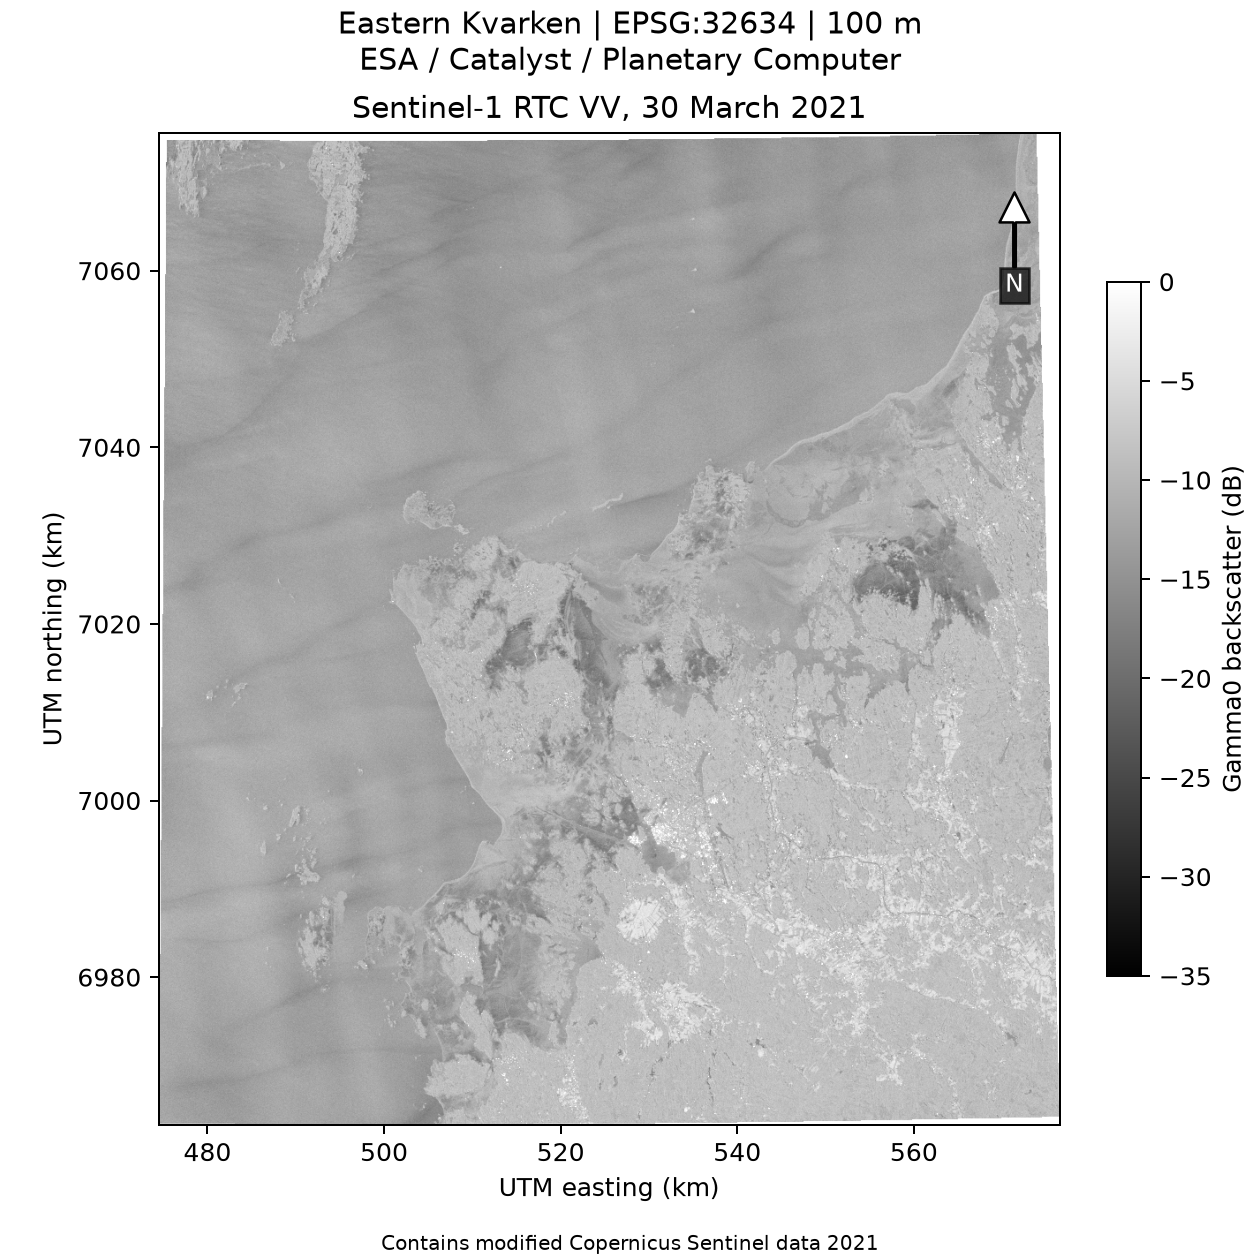
\includegraphics[width=0.95\textwidth]{../docs/research/20261019/sar_vv.png}
\caption[Sentinel-1 radar input]{Sentinel-1A VV gamma-zero input from the 30 March 2021
ESA observation. CATALYST produced the upstream RTC product, hosted and distributed as COG
assets by Microsoft Planetary Computer; the analysis also uses VH. Item identity and
processing parameters are listed in Appendix~\ref{app:repro}.}
\label{fig:sar-input}
\end{figure}

\begin{figure}[p]
\centering
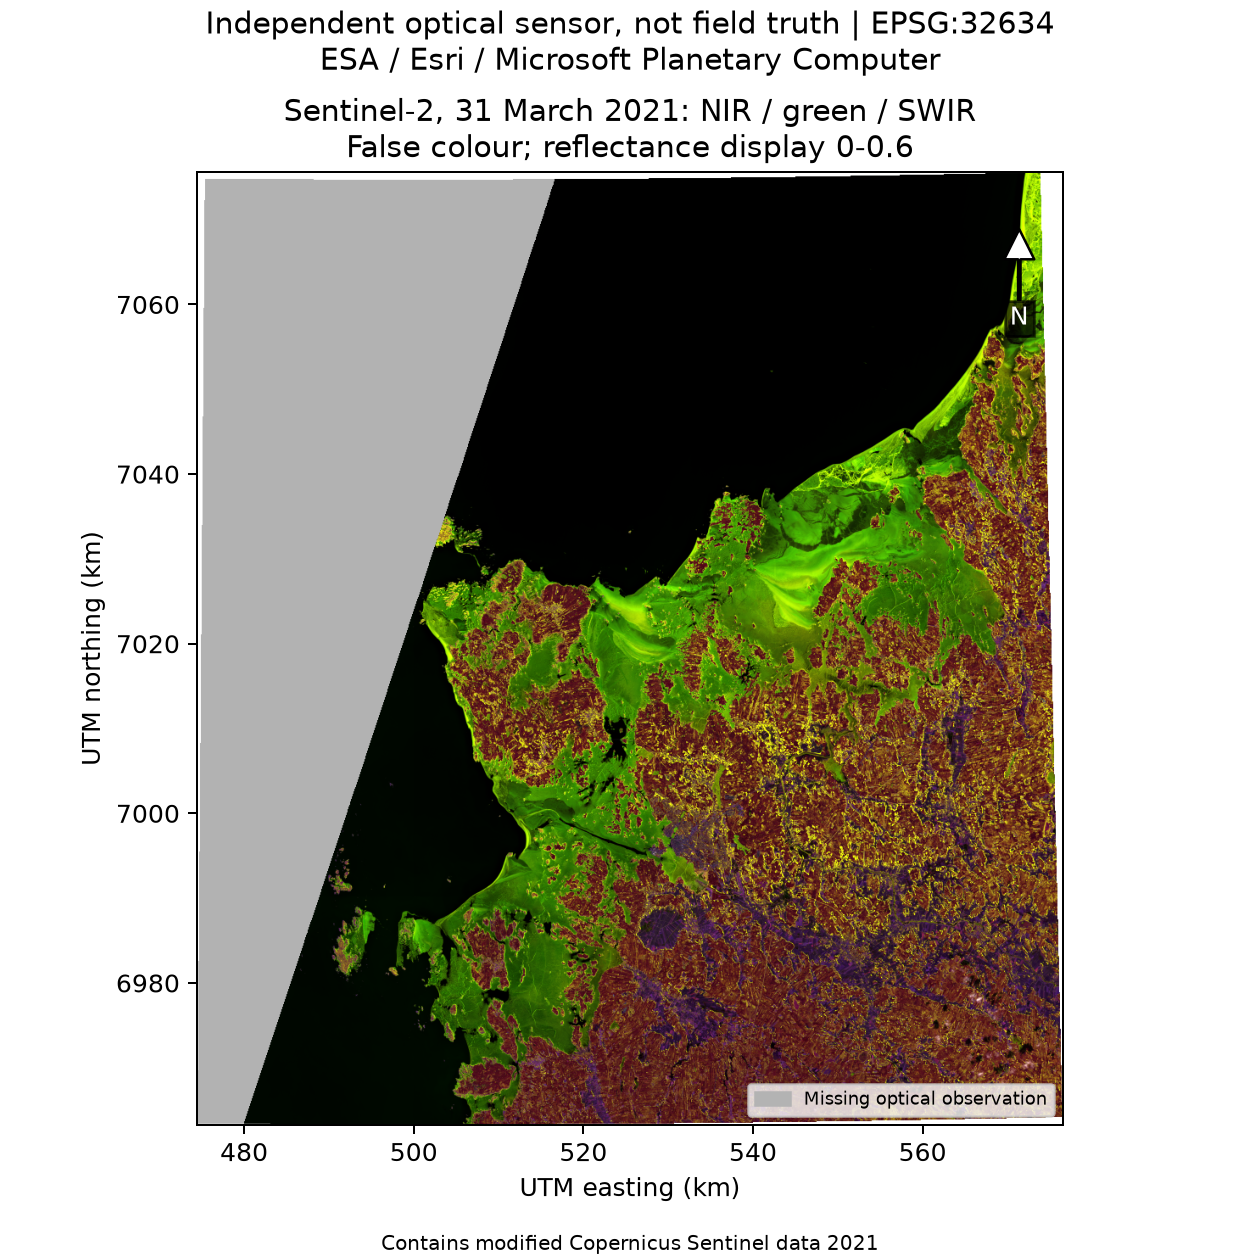
\includegraphics[width=0.95\textwidth]{../docs/research/20261019/optical_input.png}
\caption[Independent Sentinel-2 optical input]{Sentinel-2A Level-2A false-colour observation
from 31 March 2021, 17.90 hours after the radar acquisition. The STAC record identifies
ESA/Copernicus as the observation source, Esri as processor, and Microsoft Planetary Computer
as host and distributor; tile identities are listed in Appendix~\ref{app:repro}. Grey denotes
missing optical coverage.}
\label{fig:optical-input}
\end{figure}

\begin{figure}[p]
\centering
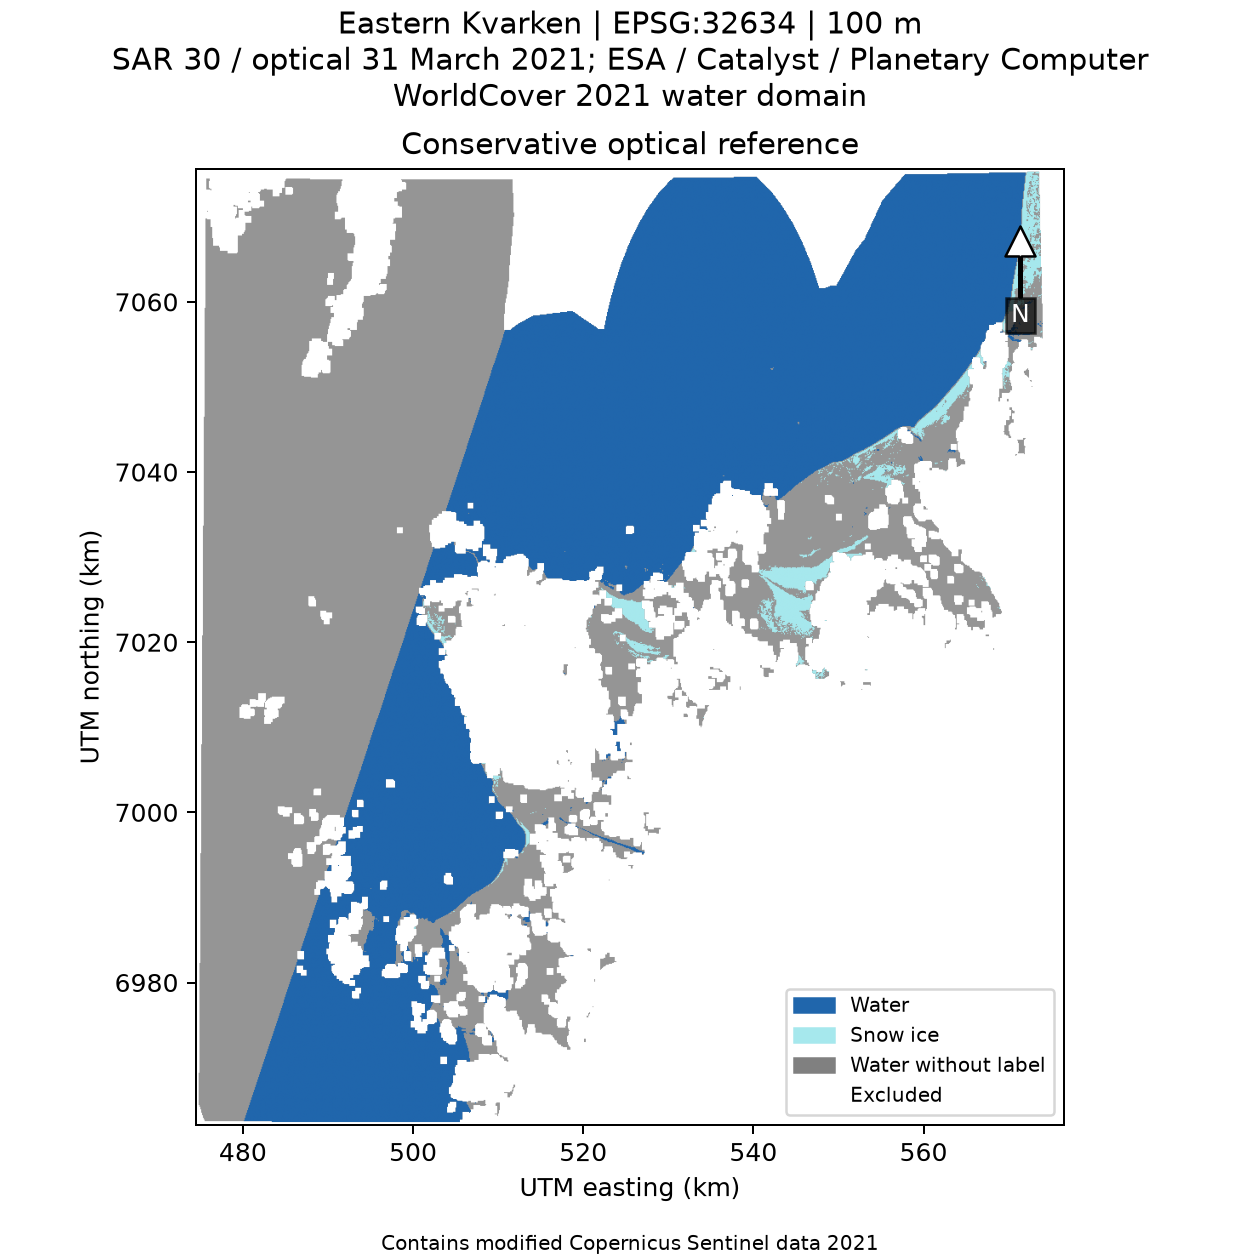
\includegraphics[width=0.95\textwidth]{../docs/research/20261019/reference.png}
\caption[Selective optical proxy reference]{Selective Sentinel-2 optical proxy labels for
dark water and bright snow-covered ice, screened with the ESA WorldCover 2021 v200
retrospective land mask. WorldCover is an annual land-cover product, not a contemporaneous
ice observation. Grey water remains unlabelled; white is outside the domain or excluded by
land/coastal screening. Product identities appear in Appendix~\ref{app:repro}.}
\label{fig:reference}
\end{figure}

\begin{figure}[p]
\centering
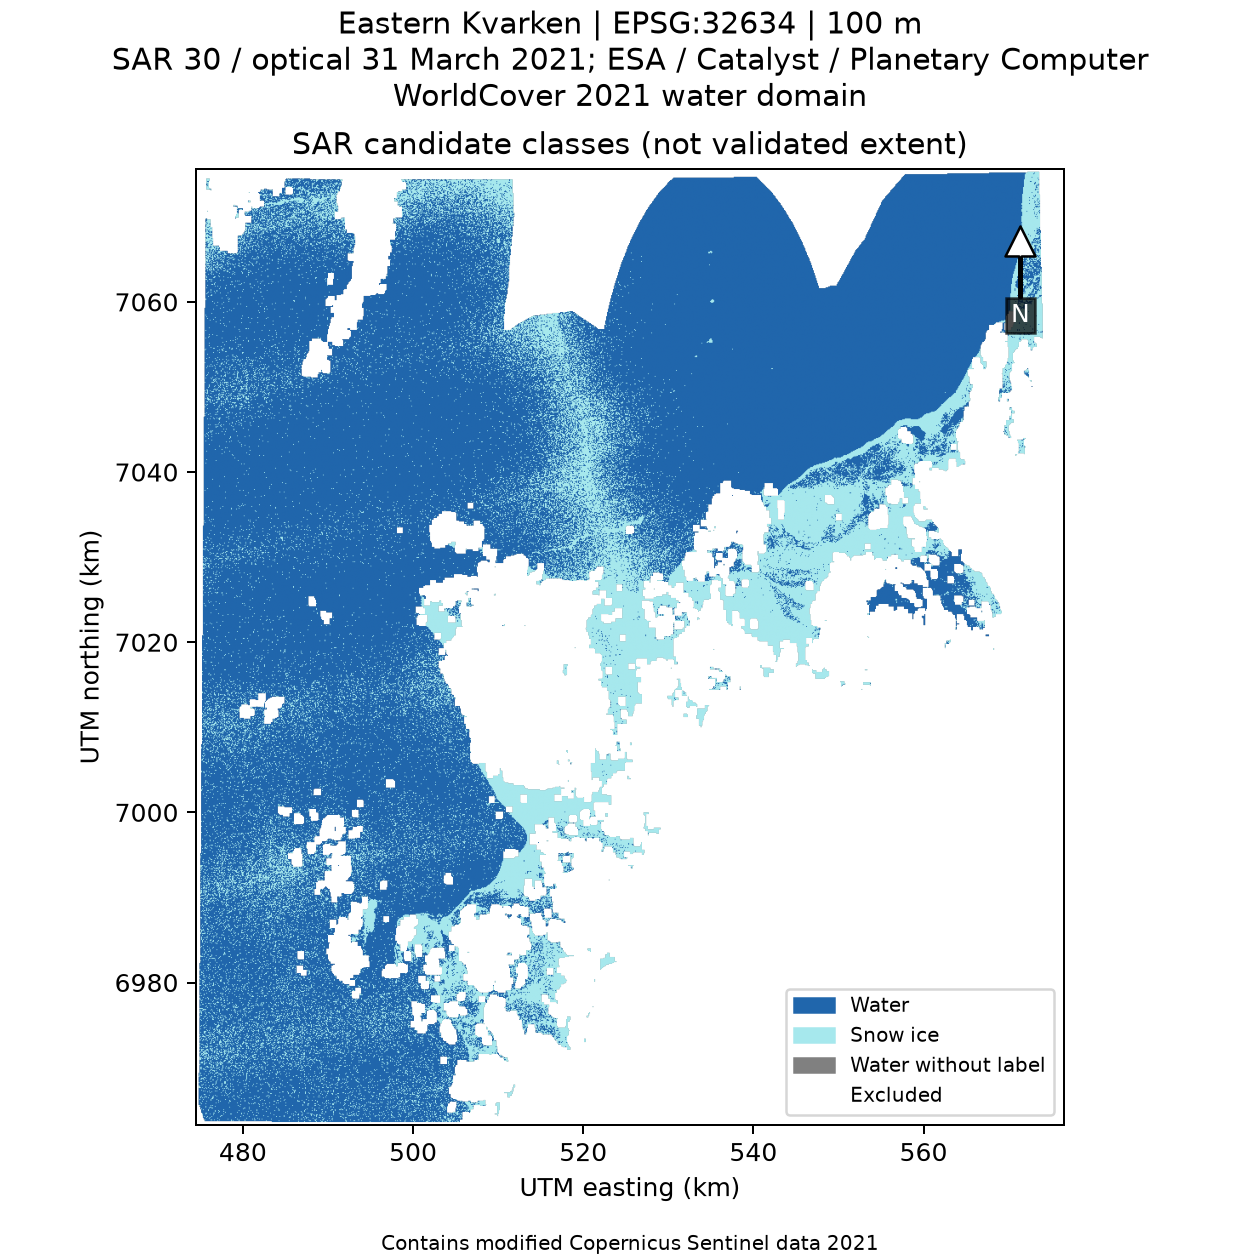
\includegraphics[width=0.95\textwidth]{../docs/research/20261019/candidate.png}
\caption[SAR candidate classes]{Scene-specific SAR candidate classes derived from ESA
Sentinel-1 observations in the upstream CATALYST RTC product hosted by Microsoft Planetary
Computer, screened with ESA WorldCover 2021 v200 and classified by the thesis-specific
VV/VH discriminant. Candidate ice is not validated sea-ice extent; 795.91~km$^2$ lacks an
optical reference label. Product identities appear in Appendix~\ref{app:repro}.}
\label{fig:candidate}
\end{figure}

\begin{figure}[p]
\centering
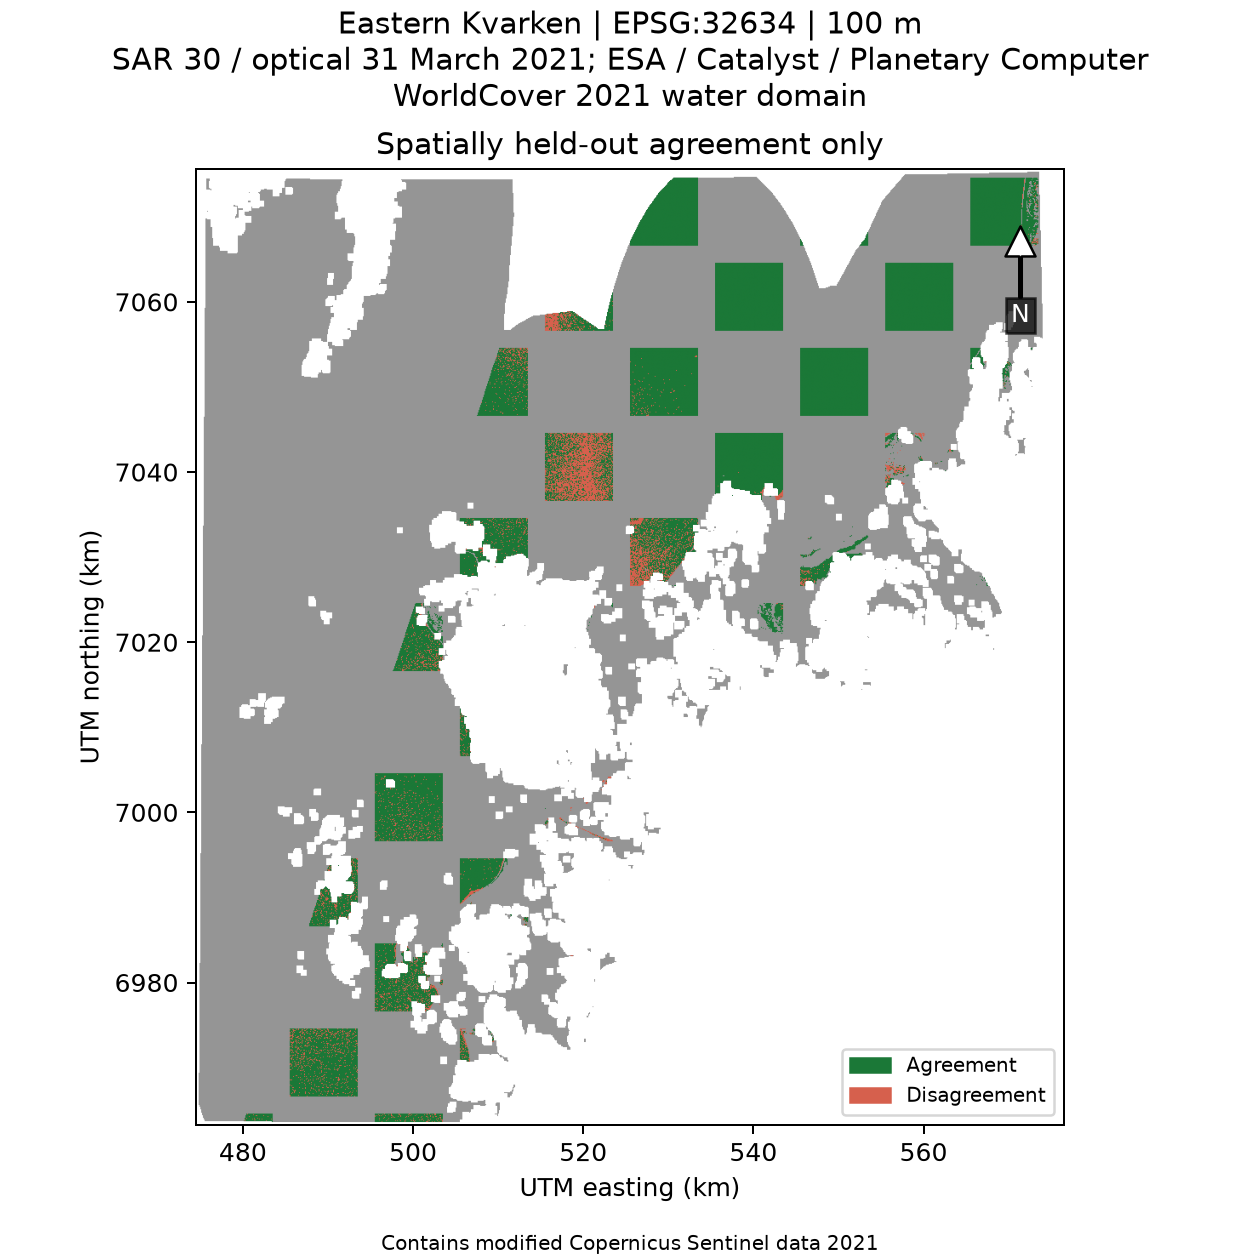
\includegraphics[width=0.95\textwidth]{../docs/research/20261019/agreement.png}
\caption[Held-out optical-reference agreement]{Held-out agreement between thesis-derived
Sentinel-1 RTC candidates and the selective Sentinel-2 optical proxy in spatially separated
checkerboard interiors. Red indicates proxy disagreement, not a field-confirmed error;
grey has no comparison. ESA supplied the observations, CATALYST produced the upstream RTC
product, and Microsoft Planetary Computer hosted and distributed the assets. Item identities
and processing parameters appear in Appendix~\ref{app:repro}.}
\label{fig:agreement}
\end{figure}

\section{Held-out comparison and majority baseline}

Native SCL purity screening leaves 281,457 water and 11,199 snow-ice reference cells.
Training uses 97,220 water and 3,469 ice cells. Held-out interiors contain 84,846 water
and 3,546 ice cells. The remaining labelled cells fall in spatially excluded edges or
other partition interiors. Table~\ref{tab:confusion} reports exact held-out counts.

\begin{table}[htbp]
\centering
\caption{Held-out confusion matrix. Rows are optical proxy labels; columns are SAR
candidate classes. Counts describe 100~m cells, not independent field observations.}
\label{tab:confusion}
\begin{tabular}{lrr}
\toprule
Optical reference & Candidate water & Candidate ice\\
\midrule
Water & 74,641 & 10,205\\
Snow-covered ice & 406 & 3,140\\
\bottomrule
\end{tabular}
\end{table}

\begin{table}[htbp]
\centering
\caption{Held-out proxy agreement. The always-water baseline is evaluated on exactly
the same cells. Undefined precision is not replaced with an invented value.}
\label{tab:agreement-metrics}
\begin{tabular}{lrr}
\toprule
Metric & SAR discriminant & Always water\\
\midrule
Ordinary agreement (\%) & 88.00 & 95.99\\
Balanced agreement (\%) & 88.26 & 50.00\\
Ice precision (\%) & 23.53 & Undefined\\
Ice recall (\%) & 88.55 & 0.00\\
Ice F1 (\%) & 37.18 & 0.00\\
\bottomrule
\end{tabular}
\end{table}

The majority baseline has higher ordinary agreement because optical water dominates
the held-out support. The discriminant detects most selected snow-ice cells, but produces
many ice predictions on proxy-water cells. Only about one in four held-out ice predictions
matches a positive optical label. It would therefore be misleading to promote the ordinary
agreement figure alone as evidence of a reliable sea-ice mapping product.

All 31 held-out blocks are retained in the machine-readable report, including blocks with
only one reference class. Their confusion counts and ordinary agreement remain defined;
balanced agreement or class recall is null where its denominator is absent. A block with
three water samples can have zero agreement, illustrating why unweighted extrema alone
are unstable. Spatially concentrated disagreements remain visible in Figure~\ref{fig:agreement}.

\section{Area, sensitivity and unsupported extrapolation}

The model predicts 1,219.28~km$^2$ of candidate ice across the analysed radar-water support.
This is a modelled candidate area, not a validated sea-ice extent.
Of this, 795.91~km$^2$ (65.28\%) has no optical proxy label at all. This area cannot be
validated by the reported held-out metrics. The selected optical ice support totals
111.99~km$^2$, but its different coverage prevents treating its difference from the full
candidate area as an ice-area error.

On the identical held-out footprint, optical positive area is 35.46~km$^2$ and candidate
positive area is 133.45~km$^2$. This supported comparison exposes substantial excess
candidate area relative to the proxy. Offsetting the discriminant by minus one, zero and
plus one produces candidate areas of 2,313.58, 1,219.28 and 695.59~km$^2$, respectively.
The large range indicates decision-boundary sensitivity. It is not a confidence interval,
and none of these offsets was selected by tuning against held-out performance.

The radar response may vary with wind, surface roughness, incidence angle and ice state.
Provider metadata reports full-scene near/far incidence angles of about 29.66--45.86 degrees;
no per-pixel incidence correction or wind record was available for this classifier.
The optical observation is later, selectively labels bright snow ice, and is not field
truth. These limitations prevent operational or universal-threshold claims. The useful
scientific result is the diagnosed failure mode and the limited, reproducible evaluation.

\section{Local and CSC infrastructure execution}

The provenance-correct final analysis began at 16:06:54 UTC on 19 October 2026. Its measured
8.54-second analysis interval includes raster calculations, publication figures and
metadata replay, but excludes source acquisition and native-mask retrieval. Timing is a
single local observation, not a CPU/GPU or local/cloud benchmark. Additional publication
layout exports can change the full command's duration without changing the numerical result.

Five actual scene records pass through bounded-active-concurrency ingestion, provenance checks, SQLite
reopening and loopback API scene/health checks. The saved run identifies Windows,
Python 3.12.15 and exact library/GDAL versions; executed Python sources and all retained
inputs/outputs have SHA-256 identities. The Git record correctly reports a dirty working
tree during execution rather than attributing uncommitted science code to the old baseline
alone.

The separate CSC replay began at 17:29:42.844271 UTC and completed at 17:29:43.815320 UTC
on 19 October 2026, with exit status zero. The full runner interval was 0.971050~s.
Its narrower ingestion timer recorded 0.199499~s, five scenes and 68,286 canonical payload
bytes, with zero failures and retries. The derived ingestion rate was 25.062840 items/s.
These two timing boundaries are distinct; neither includes VM provisioning, package
installation, raster acquisition or scientific classification.

All five catalog scene identities, all five regional query identities, all five API
identities, the health response and five provenance records matched the corresponding
local validation exactly. The Linux input bytes matched the reviewed Git blob under
SHA-256. The Windows and Linux checkouts use different line-ending conventions, so raw input-file
checksums differ across those checkouts while parsed metadata and validation results
are identical. Timestamp-bearing provenance and SQLite files are not claimed to be
byte-identical across hosts.

The retrieved compressed archive has SHA-256
\nolinkurl{c12807b646e95916540826166c02febecdec39d85034a167d90282c21b3f85df}.
The sanitized run and separate control-plane/evidence summary are retained as
\nolinkurl{docs/research/20261019/csc_pipeline_run.json} and
\nolinkurl{docs/research/20261019/csc_execution_evidence.json}.
The result demonstrates actual remote portability of the metadata/catalog/API path.
It is one small replay, not a local/cloud performance comparison, a distributed-scale
benchmark or additional validation of the sea-ice candidate map.

\section{Interpretation}

The evidence supports a dependency-free, typed metadata pipeline with bounded active concurrency,
provenance, and a reproducible regional baseline for research and teaching exercises. The result
is narrower than a production-scale platform: its demonstrated capabilities are explicit
contracts, inspectable evidence and a verified first remote metadata workflow. Live CDSE
measurements, representative raster analyses, streaming scheduling and educational evaluation
remain future work; the frozen 256-scene artifact remains unchanged as a regression reference.

\section{Live spectral-window telemetry}

To exercise the analytical path without credentials or external raster storage, the live
experiment harness runs an offline-fallback spectral-window slice after metadata ingestion. The
dated artifact \texttt{experiment\_report\_live\_20260915.json} processes one synthetic B04/B08
window of \(16\times16\) pixels, reduces it with factor \(2\) to an \(8\times8\) output, and
calculates NDVI from the reduced bands. The run records a sample NDVI of \(0.423131\), window
throughput of \(142.551675\) windows per second, and a traced Python peak allocation of 14,136
bytes.

These values complement, rather than replace, the frozen 256-scene baseline. The baseline's
220.819653 items per second measures metadata ingestion, provenance, and catalog indexing,
whereas the live telemetry measures a numerical window transformation. Their units and work
sets differ, so comparing the numbers as a single performance ranking would be invalid. The
useful result is that both paths produce dated, inspectable evidence under the same offline
fallback contract, while authenticated CDSE execution can later substitute real response and
raster-window observations.

The telemetry also verifies two processing invariants. First, the factor-two reduction uses the
actual arithmetic mean of every block, including edge blocks, so constant radiometric fields do
not darken. Second, B04 and B08 use the same window and factor before NDVI evaluation, preserving
pixel correspondence. The reported peak memory is Python allocation measured by
\texttt{tracemalloc}; it excludes native decoder buffers and remote transfer caches.

\chapter{Analysis}

\section{Analysis of RQ1: provider-neutral validation and provenance}

RQ1 asks how heterogeneous STAC and CDSE-shaped metadata can be validated and transformed into a transport-neutral scene model while preserving provenance. The implemented answer is a boundary-validation step followed by transformation into the provider-neutral \texttt{EOScene} model. Raw canonical payloads are stored separately under SHA-256 identities and accompanied by append-only manifest records.

This design separates two needs that are often conflated: convenient normalized state for queries and immutable source evidence for audit. The catalog can evolve independently from the raw evidence without erasing what arrived from the provider. The evidence is strong within the implemented schema and fixtures, but it does not establish compatibility with every EO provider or every STAC extension.

\section{Analysis of RQ2: bounded concurrency and failure recovery}

RQ2 concerns bounded asynchronous work and selective recovery. The implementation uses an explicit semaphore to constrain active processing and persistence.
Its current batch gather still schedules a coroutine for each supplied item; the bound is on
active work, not on arbitrary response-list memory. The real-data replay supplies five items. Tests cover timeout, HTTP 429, token expiry, exhausted retries, malformed payloads, and invalid token responses.

The central result is behavioral rather than statistical: the system distinguishes transient transport conditions from deterministic input failures and applies retry logic only to the former. The frozen benchmark itself observed zero failures and zero retries, so it cannot be used to estimate a production recovery rate. Recovery claims therefore rest on controlled tests, not on the benchmark field \texttt{failure\_recovery\_ratio}.

\section{Analysis of RQ3: SQLite catalog effectiveness}

RQ3 asks whether a dependency-free SQLite catalog is effective for the local regional-query workload. The implementation supports regional, temporal, quality, and platform filters. Bounding-box predicates reduce candidate sets before deterministic geometry checks, while WAL and transaction tests cover local reader/writer behavior.

The frozen benchmark records a 9.117 ms spatial-query value. This value is useful as a local regression point because it was produced by a preserved workload, but it is not a general latency guarantee. The evidence supports SQLite as a practical single-node baseline with low operational overhead. It does not support claims about multi-node or distributed scalability.

\section{Analysis of RQ4: reproducibility}

RQ4 asks which measurements and artifacts are sufficient to make the offline pipeline baseline reproducible. The project combines checked-in fixtures, a frozen experiment report, explicit benchmark configuration, versioned source, CI, deterministic report schemas, and dated additive live/fallback artifacts.

The main reproducibility result is therefore the evidence chain rather than any single metric. The system records which mode ran, what input class was used, which metrics were emitted, and which artifact supports a thesis claim. The approach cannot guarantee identical timing on different hardware, but it makes differences inspectable.

\section{Analysis of RQ5: a traceable scientific application}

The Sentinel-1 application demonstrates why metadata infrastructure matters beyond a
catalog benchmark. Actual scene identities lead to authenticated-by-checksum cached pixels,
aligned processing, maps, a held-out comparison and a persistent metadata/API replay.
Native categorical masks and common optical tile ownership became necessary only when the
pipeline encountered real spatial footprints. Infrastructure tests alone would not have
exposed the poor positive precision of the radar classifier.

The scientific answer is narrower than reliable ice-extent monitoring. Conservative
optical labels support a reproducible agreement test, but the classifier's positive
precision is low and most candidate ice area lacks a reference label. The experiment
demonstrates an auditable application and its limitations, not a validated operational
ice product. Independent physical observations, wind/incidence analysis and multiple dates
are needed to establish broader scientific performance. CSC execution is still unverified.

\section{Cross-cutting interpretation}

Across the five questions, the strongest result is the explicit connection between software contracts and claim boundaries. Provider behavior is isolated, concurrency is bounded, raw evidence is retained, spatial assumptions are stated, and experiment artifacts are preserved. This makes the baseline suitable for regression-oriented research and educational demonstrations.

At the same time, the evidence remains deliberately narrower than a production evaluation. Real authenticated CDSE performance, large raster workloads, distributed execution, and learning outcomes remain future research tasks.

\chapter{Discussion}

\section{Scientific and engineering contribution}

The contribution is the connection between provider access, validated metadata, provenance,
bounded active concurrency, spatial persistence and a concrete application. STAC describes assets,
OGC standards provide an interoperability context, and CDSE provides a relevant Copernicus
access environment \citep{stac-spec,ogc-api-features,cdse,kovacs2026cdse}. The thesis does
not invent metadata catalogs, OAuth2, SQLite or a new remote-sensing classifier.

Actual Sentinel-1 and Sentinel-2 observations make the practical contribution observable.
Scene identities lead to retained pixels, aligned processing, maps, spatial holdouts and
a persistent metadata/API replay. Native categorical masks and common optical tile ownership
became necessary when processing real spatial footprints. Infrastructure tests alone would
not have exposed the low positive precision of the radar classifier.

The standard-library baseline reduces installation variability; the optional science
environment supplies capabilities that would be inappropriate to reimplement inside it.
An embedded catalog is easy to reproduce but is not a distributed service. These are
explicit scope choices, not universal recommendations.

\section{What the scientific comparison establishes}

The discriminant recognises many selectively labelled snow-ice cells, but its ice precision
is low. The always-water baseline achieves higher ordinary agreement because the reference
is strongly imbalanced. Balanced agreement, confusion counts, supported-area comparison and
spatial maps are therefore needed together. A plausible-looking candidate map is insufficient.

Sentinel-2 supplies an independent sensor, not field truth \citep{drusch2012sentinel}.
The proxy rules preferentially retain bright snow ice and dark water. Thin, wet, dark or
cloud-obscured ice may be omitted or mislabelled. The 17.90-hour mismatch also permits
physical changes and displacement. These effects prevent interpreting every disagreement
as a Sentinel-1 classification error.

Radar calibration and terrain correction have an established methodological basis
\citep{small2011,pc-s1-rtc}. They do not remove the need to investigate wind, ice state and
incidence-angle effects in a downstream sea-ice classifier. No such universal correction
or threshold is established here. Official Baltic ice charts would provide useful context,
but their documented SAR inputs prevent treating them as fully independent Sentinel-1
ground truth \citep{cmems-ice-pum}.

\section{Reproducibility and threats to validity}

\subsection{Internal validity}

The historical benchmark is controlled and synthetic. Its timings are single observations
rather than repeated distributions. Filesystem cache state, scheduling, temporary storage
and background processes can affect them. Automated failure injection establishes particular
behaviours, not production failure probabilities.

The real-data evaluation uses separated blocks, but only one radar/optical pair. Spatial
autocorrelation can persist across blocks. Test pixels are not independent field samples.
All single-class blocks are retained instead of suppressing their errors; undefined metrics
are explicitly null. The model and proxy rules were not tuned against held-out performance.

\subsection{Construct and external validity}

Metadata throughput is not raster bandwidth; local query latency is not deployed end-user
latency. Candidate ice area is not validated total ice extent. Most positive candidate area
has no optical label, and reference selection limits extrapolation. The largest connected
water component is an approximation, not an official marine boundary. Coastal erosion
removes potentially important coastal ice as well as contamination.

WorldCover is an annual 2021 retrospective mask, partly informed by Sentinel-1 and Sentinel-2.
It can include information acquired after March and is not independent ice validation.
One selected eastern-Kvarken case does not establish performance across seasons, sensors,
or the whole Kvarken strait. No students or educational learning outcomes were evaluated.

\subsection{Reproducibility limits}

The frozen fixtures, reports and actual-data manifests make claims inspectable. The
real-data run additionally records unsigned endpoints, parameters, dependency/GDAL versions
and executed-source hashes. Checksums identify retained reprojected windows, not complete
original SAFE packages. A changed provider product or access policy may prevent exact
retrieval later. Timing and provenance timestamps are not expected to reproduce bitwise.

\section{Implications for Kvarken Space Center and CSC}

A modest infrastructure can make provenance and evaluation explicit before becoming a
production platform. The application shows why this matters: it preserves a weak result
and exposes its limits rather than promoting a map without examining support.
The study does not document a formal organisational requirements survey or production service.
The implemented fixture exercises, validation, provenance inspection, spatial queries,
read-only API, and local raster evaluation provide material for teaching. The CSC replay
extends that path to a first remote metadata workflow. The project did not evaluate student
learning or compare teaching outcomes.

The authenticated CSC replay provides a second execution environment for the five-scene
metadata path. Its source, input and output identities and exact local/remote query
comparison make the deployment auditable. This is a portability demonstration, not
distributed processing: one small CPU VM ran an embedded catalog and a loopback API.
Its single-run timing cannot establish cloud speedup, reliability or production scale.
It does not alter the locally measured classifier precision or unsupported candidate area.
Allas and Roihu are not required merely to make the architecture appear larger.

\section{Scientific and submission boundaries}

Further acquisitions, temporally matched independent observations, wind information and
incidence-angle stratification are needed before broader ice-mapping claims. The current
application provides diagnostic scientific evaluation, not operational validation.
A successful local PDF build also does not establish Google Docs synchronization, author
approval, supervisor acceptance, Turnitin clearance or institutional submission readiness.
Those gates remain open in the delivery record.

\chapter{Conclusion and Future Work}

\section{Conclusion}

This thesis connects an auditable EO metadata infrastructure to an actual satellite-data
application in eastern Kvarken. The core combines typed boundaries, injectable transport,
bounded active ingestion, content-addressed provenance, a WAL-enabled SQLite spatial catalog,
quality filters and a read-only educational interface. An optional scientific environment
adds observed Sentinel-1 and Sentinel-2 raster windows, WorldCover screening, candidate maps
and quantitative proxy evaluation without changing the lightweight runtime requirement.

The application addresses the earlier absence of practical pixel processing. It also
shows why scientific validation cannot be replaced by infrastructure success. Positive
radar candidates have low precision against the selected optical proxy, and most candidate
ice area has no reference label. The output must not be described as reliable total
sea-ice extent. A separate CSC cPouta metadata replay verified the same five scene
identities, persistent provenance, regional queries and loopback API as the local run.

\section{Answers to the research questions}

\subsection{RQ1: provider-neutral metadata and provenance}

Validate provider JSON at the boundary, transform accepted items into a frozen scene model,
and retain canonical raw payloads independently under SHA-256 identities. Append-only
records preserve source and acquisition context while SQLite supports convenient queries.
The application exposed the importance of distinguishing geographic STAC geometry from
the projected raster CRS and of preserving each optical item's own source endpoint.

\subsection{RQ2: bounded active work and recovery}

A semaphore limits active processing and persistence. Bounded retries distinguish transient
timeouts and throttling from malformed inputs. The current batch gather still schedules
one coroutine per supplied item; it is not a proof of bounded scheduling memory for an
arbitrarily large response list. The application replay uses five captured scene records.
Failure-oriented tests establish particular behaviours rather than a production recovery rate.

\subsection{RQ3: regional catalog behaviour}

Bounding-box predicates followed by deterministic geometry checks support regional,
temporal, platform and quality queries in a compact local catalog. WAL and reopening tests
cover committed-state durability and mixed reader/writer behaviour. The historical 9.117~ms
query observation is a local regression point, not a latency guarantee or distributed benchmark.

\subsection{RQ4: reproducible evidence}

Version fixtures, parameters, source, reports and validation commands together. Keep the
frozen 256-scene benchmark explicitly synthetic and the 20260915 artifact explicitly
offline fallback. Add actual-data manifests, retained-window checksums and source/environment
identities rather than overwriting historical comparisons. Reproducibility here means
inspectable computation and provenance, not identical wall-clock timings.

\subsection{RQ5: a traceable practical application}

Actual observations can be connected to cached pixels, preprocessing, candidate classification,
independent-sensor proxy comparison and the existing catalog/API. Shared optical tile
ownership and native categorical class purity are necessary to avoid misleading reference
construction. The held-out comparison diagnoses a weak classifier; it does not establish
accurate total ice extent or universal SAR thresholds. The CSC replay supplies genuine
remote infrastructure evidence, not a second scientific validation experiment.

\section{Contributions and limitations}

The contribution is methodological and software-oriented: small, inspectable contracts link
provider standards to reproducible local research. The real application adds a practical
test of those contracts and retains its negative findings. It is not a new SAR algorithm,
a field-validated sea-ice product, a production cloud service or an educational outcome study.
The annual mask, selective proxy labels, acquisition mismatch and single-scene design
constrain the scientific conclusions.

\section{Immediate and future work}

The CSC demonstration retained verified project and instance identity, deployed source,
remote timestamps, commands, output checksums and health results. Its temporary instances
and floating IP were released after evidence retrieval. Future deployments should retain
that evidence boundary and keep APIs on loopback rather than expose an unprotected public
service. Repeated equivalent workloads are needed before local/cloud performance claims.

Scientific follow-up should use several radar acquisitions, independent temporally matched
observations, wind records and incidence-angle analysis. The optical proxy needs validation
of its own, especially for thin or dark ice. Candidate-area uncertainty requires stronger
evidence than the reported decision-offset sensitivity.

Longer-term engineering work includes bounded scheduling for large streaming batches,
repeated resource measurements, continuous authenticated CDSE ingestion, backup/restore drills
and appropriately governed distributed storage. These extensions should preserve the
offline regression path and immutable evidence.

\section{Closing statement}

The work connects real satellite analysis with a verified CSC metadata deployment while
exposing a scientific failure mode. Its auditable evidence supports infrastructure
portability, not operational ice mapping. Author review and supervisor approval remain required.


\printbibliography[heading=bibintoc,title={References}]

\appendix
\chapter{Disclosure of AI-Assisted Work}

\section{Tool, purpose and scope}

The October 2026 revision used an AI assistant using Copilot SDK in VS Code
\citep{copilot}. Assistance was substantial: repository recovery, source discovery,
scientific-method assessment, Python implementation, tests, raster acquisition commands,
plotting code, statistical reporting, manuscript restructuring, language editing, citation
checks and delivery documentation. The exact underlying model is not independently recorded
and is not asserted here. An earlier recovered draft attributed assistance to ChatGPT; that
historical attribution has not been independently verified.

The manuscript is an AI-assisted working draft. The author's personal examination and
acceptance of all revised claims, code, references and text remain required. Neither this
appendix nor an automated build establishes that the author has already performed that
review. The author retains responsibility for the submitted thesis and must complete the
university's AI reporting requirements before submission \citep{uwasa-writing}.

\section{Representative prompts and affected material}

The principal user prompt requested: ``Build and execute the real workflow'', ``Do not
assume that one universal backscatter threshold can reliably distinguish sea ice'', and
``Never invent scientific results, datasets, evaluations, citations, plagiarism scores or
reviewer approvals.'' These instructions informed Chapters 5--6 and the real-data scripts.
The revision request also asked for actual CSC execution and honest identification of
external blockers. It did not authorize invented cloud evidence.

The independent code/science review prompt requested a read-only audit of the scientific
code, input manifests, maps and results, including preprocessing, validation leakage,
metrics, provenance and claim boundaries. Its findings led to shared optical tile
ownership, native categorical class-purity masks, complete single-class block reporting,
source-specific provenance and executed-source checksums.

The mapping prompt requested genuine satellite inputs, processed maps, independent
comparison figures, meaningful geography, legends, units, coordinate reference and source
information. AI assistance generated plotting and processing code; the maps are computed
from recorded satellite pixels, not image-synthesis outputs. Figure captions identify this
assistance. Detailed user prompts and execution history remain in the agent session, which
is not itself an independently archived research dataset.

\section{Verification and remaining responsibility}

Automated tests exercise masking, power conversion, alignment, classification calculations,
metrics and provenance. Saved raster values are cross-checked against reported confusion
counts and areas. Acquisition and derived-output checksums identify retained files; DOI
metadata and authoritative documentation support the cited methods. A separate AI reviewer
recomputed the initial confusion matrix and identified concrete defects, which were
addressed before the reported reviewed run. This is computational cross-checking, not
human peer review or university approval.

No AI output is treated as an observation, field label, supervisor approval, Turnitin
result or CSC execution record. Local maps and numerical reports derive from actual
satellite inputs, with selective optical proxy labels clearly distinguished from ground
truth. The unresolved CSC execution and Google Docs synchronization are reported as
blocked. Before submission the author must verify this disclosure against the actual
tools used and complete any programme-specific declaration or signature.

\chapter{Reproducibility and Claim Boundaries}

\section{Historical evidence}

\begin{itemize}
\item Package 0.1.0 is the released baseline; its runtime has no third-party dependencies.
\item The historical release recorded 53 passing tests; later additions are separate checkpoints.
\item The frozen benchmark has 256 synthetic scenes at concurrency eight.
\item Its 220.819653 items/s throughput is local metadata-path performance, not CDSE or raster bandwidth.
\item Its 9.117~ms query measurement is not a general latency guarantee.
\item The 20260915 artifact is \texttt{offline-fallback} / \texttt{offline-fixture}, not a live CDSE run.
\item The earlier range/NDVI slice uses aligned fixture arrays. The optional science environment
separately processes actual GeoTIFF windows; it is not a general-purpose SAR processor.
\item The educational API was tested, but learning outcomes and distributed scale were not evaluated.
\end{itemize}

\section{Actual-data reproduction}

The canonical configuration and small evidence files are in
\texttt{docs/research/20261019/}; large raster windows remain in ignored local storage.
The following commands run from the repository root. Enter each on one line in PowerShell.
Use a new output directory for each completed analysis.

\begin{verbatim}
python -m pip install -e ".[dev,science]"
python -m kvarken_eo.case_study --help
python -m pytest
python -m ruff check .
python -m ruff format --check .
python -m kvarken_eo verify-health
\end{verbatim}

For fresh acquisition, invoke \texttt{python -m kvarken\_eo.case\_study} with
\texttt{--config} \nolinkurl{docs/research/20261019/case_config.json},
\texttt{--inputs-dir} \nolinkurl{data/seaice_reproduction}, and
\texttt{--output-dir} \nolinkurl{outputs/seaice_reproduction}; use the platform's path separators.
For another analysis of those verified inputs, omit the configuration and add
\texttt{--reuse-inputs}, choosing a different output directory.

Acquisition requires live source access and temporary read-only signing tokens.
Reuse checks cached hashes and contacts only the local API. The interrupted initial
acquisition is retained. Native categorical coverage corrections have a supplemental,
immutable quality-mask manifest linked to the original input manifest.
The native-mask preparation option is required only when extending an older cache lacking
those masks, not for ordinary fresh acquisition.

Numerical results are deterministic for the retained inputs and parameters. Timing,
timestamps and catalog/provenance bytes may change between runs. Executed-source hashes
and package/GDAL versions identify the actual implementation when Git was dirty;
the old base commit alone does not contain that extension. The published report lists
all held-out blocks and uses null for undefined metrics.

\section{Environment and acceptance gates}

Raster processing ran on the local Windows CPU, not the GPU or CSC. No authenticated
CDSE pixel download is claimed. A separate five-scene metadata replay executed on CSC
cPouta with verified source, environment and retrieved output hashes. The evidence is in
\nolinkurl{docs/research/20261019/csc_execution_evidence.json}; it does not include remote
raster classification. The repository delivery
report records the secure-access prerequisites and submission sequence. Google Docs
synchronization, personal author review and all university approvals remain separate gates.


\end{document}
